% Preliminary draft. Tables in tables/ and figures in figures/ are generated by make_tables.py
% from results/poc-tev1-0.8b (run `uv run python paper/make_tables.py --run poc-tev1-0.8b --model tev1:0.8b --bench bench-np4`).
\documentclass[10pt]{article}
\usepackage[preprint]{tmlr}

%%%%% NEW MATH DEFINITIONS %%%%%

\usepackage{amsmath,amsfonts,bm}

% Mark sections of captions for referring to divisions of figures
\newcommand{\figleft}{{\em (Left)}}
\newcommand{\figcenter}{{\em (Center)}}
\newcommand{\figright}{{\em (Right)}}
\newcommand{\figtop}{{\em (Top)}}
\newcommand{\figbottom}{{\em (Bottom)}}
\newcommand{\captiona}{{\em (a)}}
\newcommand{\captionb}{{\em (b)}}
\newcommand{\captionc}{{\em (c)}}
\newcommand{\captiond}{{\em (d)}}

% Highlight a newly defined term
\newcommand{\newterm}[1]{{\bf #1}}


% Figure reference, lower-case.
\def\figref#1{figure~\ref{#1}}
% Figure reference, capital. For start of sentence
\def\Figref#1{Figure~\ref{#1}}
\def\twofigref#1#2{figures \ref{#1} and \ref{#2}}
\def\quadfigref#1#2#3#4{figures \ref{#1}, \ref{#2}, \ref{#3} and \ref{#4}}
% Section reference, lower-case.
\def\secref#1{section~\ref{#1}}
% Section reference, capital.
\def\Secref#1{Section~\ref{#1}}
% Reference to two sections.
\def\twosecrefs#1#2{sections \ref{#1} and \ref{#2}}
% Reference to three sections.
\def\secrefs#1#2#3{sections \ref{#1}, \ref{#2} and \ref{#3}}
% Reference to an equation, lower-case.
\def\eqref#1{equation~\ref{#1}}
% Reference to an equation, upper case
\def\Eqref#1{Equation~\ref{#1}}
% A raw reference to an equation---avoid using if possible
\def\plaineqref#1{\ref{#1}}
% Reference to a chapter, lower-case.
\def\chapref#1{chapter~\ref{#1}}
% Reference to an equation, upper case.
\def\Chapref#1{Chapter~\ref{#1}}
% Reference to a range of chapters
\def\rangechapref#1#2{chapters\ref{#1}--\ref{#2}}
% Reference to an algorithm, lower-case.
\def\algref#1{algorithm~\ref{#1}}
% Reference to an algorithm, upper case.
\def\Algref#1{Algorithm~\ref{#1}}
\def\twoalgref#1#2{algorithms \ref{#1} and \ref{#2}}
\def\Twoalgref#1#2{Algorithms \ref{#1} and \ref{#2}}
% Reference to a part, lower case
\def\partref#1{part~\ref{#1}}
% Reference to a part, upper case
\def\Partref#1{Part~\ref{#1}}
\def\twopartref#1#2{parts \ref{#1} and \ref{#2}}

\def\ceil#1{\lceil #1 \rceil}
\def\floor#1{\lfloor #1 \rfloor}
\def\1{\bm{1}}
\newcommand{\train}{\mathcal{D}}
\newcommand{\valid}{\mathcal{D_{\mathrm{valid}}}}
\newcommand{\test}{\mathcal{D_{\mathrm{test}}}}

\def\eps{{\epsilon}}


% Random variables
\def\reta{{\textnormal{$\eta$}}}
\def\ra{{\textnormal{a}}}
\def\rb{{\textnormal{b}}}
\def\rc{{\textnormal{c}}}
\def\rd{{\textnormal{d}}}
\def\re{{\textnormal{e}}}
\def\rf{{\textnormal{f}}}
\def\rg{{\textnormal{g}}}
\def\rh{{\textnormal{h}}}
\def\ri{{\textnormal{i}}}
\def\rj{{\textnormal{j}}}
\def\rk{{\textnormal{k}}}
\def\rl{{\textnormal{l}}}
% rm is already a command, just don't name any random variables m
\def\rn{{\textnormal{n}}}
\def\ro{{\textnormal{o}}}
\def\rp{{\textnormal{p}}}
\def\rq{{\textnormal{q}}}
\def\rr{{\textnormal{r}}}
\def\rs{{\textnormal{s}}}
\def\rt{{\textnormal{t}}}
\def\ru{{\textnormal{u}}}
\def\rv{{\textnormal{v}}}
\def\rw{{\textnormal{w}}}
\def\rx{{\textnormal{x}}}
\def\ry{{\textnormal{y}}}
\def\rz{{\textnormal{z}}}

% Random vectors
\def\rvepsilon{{\mathbf{\epsilon}}}
\def\rvtheta{{\mathbf{\theta}}}
\def\rva{{\mathbf{a}}}
\def\rvb{{\mathbf{b}}}
\def\rvc{{\mathbf{c}}}
\def\rvd{{\mathbf{d}}}
\def\rve{{\mathbf{e}}}
\def\rvf{{\mathbf{f}}}
\def\rvg{{\mathbf{g}}}
\def\rvh{{\mathbf{h}}}
\def\rvu{{\mathbf{i}}}
\def\rvj{{\mathbf{j}}}
\def\rvk{{\mathbf{k}}}
\def\rvl{{\mathbf{l}}}
\def\rvm{{\mathbf{m}}}
\def\rvn{{\mathbf{n}}}
\def\rvo{{\mathbf{o}}}
\def\rvp{{\mathbf{p}}}
\def\rvq{{\mathbf{q}}}
\def\rvr{{\mathbf{r}}}
\def\rvs{{\mathbf{s}}}
\def\rvt{{\mathbf{t}}}
\def\rvu{{\mathbf{u}}}
\def\rvv{{\mathbf{v}}}
\def\rvw{{\mathbf{w}}}
\def\rvx{{\mathbf{x}}}
\def\rvy{{\mathbf{y}}}
\def\rvz{{\mathbf{z}}}

% Elements of random vectors
\def\erva{{\textnormal{a}}}
\def\ervb{{\textnormal{b}}}
\def\ervc{{\textnormal{c}}}
\def\ervd{{\textnormal{d}}}
\def\erve{{\textnormal{e}}}
\def\ervf{{\textnormal{f}}}
\def\ervg{{\textnormal{g}}}
\def\ervh{{\textnormal{h}}}
\def\ervi{{\textnormal{i}}}
\def\ervj{{\textnormal{j}}}
\def\ervk{{\textnormal{k}}}
\def\ervl{{\textnormal{l}}}
\def\ervm{{\textnormal{m}}}
\def\ervn{{\textnormal{n}}}
\def\ervo{{\textnormal{o}}}
\def\ervp{{\textnormal{p}}}
\def\ervq{{\textnormal{q}}}
\def\ervr{{\textnormal{r}}}
\def\ervs{{\textnormal{s}}}
\def\ervt{{\textnormal{t}}}
\def\ervu{{\textnormal{u}}}
\def\ervv{{\textnormal{v}}}
\def\ervw{{\textnormal{w}}}
\def\ervx{{\textnormal{x}}}
\def\ervy{{\textnormal{y}}}
\def\ervz{{\textnormal{z}}}

% Random matrices
\def\rmA{{\mathbf{A}}}
\def\rmB{{\mathbf{B}}}
\def\rmC{{\mathbf{C}}}
\def\rmD{{\mathbf{D}}}
\def\rmE{{\mathbf{E}}}
\def\rmF{{\mathbf{F}}}
\def\rmG{{\mathbf{G}}}
\def\rmH{{\mathbf{H}}}
\def\rmI{{\mathbf{I}}}
\def\rmJ{{\mathbf{J}}}
\def\rmK{{\mathbf{K}}}
\def\rmL{{\mathbf{L}}}
\def\rmM{{\mathbf{M}}}
\def\rmN{{\mathbf{N}}}
\def\rmO{{\mathbf{O}}}
\def\rmP{{\mathbf{P}}}
\def\rmQ{{\mathbf{Q}}}
\def\rmR{{\mathbf{R}}}
\def\rmS{{\mathbf{S}}}
\def\rmT{{\mathbf{T}}}
\def\rmU{{\mathbf{U}}}
\def\rmV{{\mathbf{V}}}
\def\rmW{{\mathbf{W}}}
\def\rmX{{\mathbf{X}}}
\def\rmY{{\mathbf{Y}}}
\def\rmZ{{\mathbf{Z}}}

% Elements of random matrices
\def\ermA{{\textnormal{A}}}
\def\ermB{{\textnormal{B}}}
\def\ermC{{\textnormal{C}}}
\def\ermD{{\textnormal{D}}}
\def\ermE{{\textnormal{E}}}
\def\ermF{{\textnormal{F}}}
\def\ermG{{\textnormal{G}}}
\def\ermH{{\textnormal{H}}}
\def\ermI{{\textnormal{I}}}
\def\ermJ{{\textnormal{J}}}
\def\ermK{{\textnormal{K}}}
\def\ermL{{\textnormal{L}}}
\def\ermM{{\textnormal{M}}}
\def\ermN{{\textnormal{N}}}
\def\ermO{{\textnormal{O}}}
\def\ermP{{\textnormal{P}}}
\def\ermQ{{\textnormal{Q}}}
\def\ermR{{\textnormal{R}}}
\def\ermS{{\textnormal{S}}}
\def\ermT{{\textnormal{T}}}
\def\ermU{{\textnormal{U}}}
\def\ermV{{\textnormal{V}}}
\def\ermW{{\textnormal{W}}}
\def\ermX{{\textnormal{X}}}
\def\ermY{{\textnormal{Y}}}
\def\ermZ{{\textnormal{Z}}}

% Vectors
\def\vzero{{\bm{0}}}
\def\vone{{\bm{1}}}
\def\vmu{{\bm{\mu}}}
\def\vtheta{{\bm{\theta}}}
\def\va{{\bm{a}}}
\def\vb{{\bm{b}}}
\def\vc{{\bm{c}}}
\def\vd{{\bm{d}}}
\def\ve{{\bm{e}}}
\def\vf{{\bm{f}}}
\def\vg{{\bm{g}}}
\def\vh{{\bm{h}}}
\def\vi{{\bm{i}}}
\def\vj{{\bm{j}}}
\def\vk{{\bm{k}}}
\def\vl{{\bm{l}}}
\def\vm{{\bm{m}}}
\def\vn{{\bm{n}}}
\def\vo{{\bm{o}}}
\def\vp{{\bm{p}}}
\def\vq{{\bm{q}}}
\def\vr{{\bm{r}}}
\def\vs{{\bm{s}}}
\def\vt{{\bm{t}}}
\def\vu{{\bm{u}}}
\def\vv{{\bm{v}}}
\def\vw{{\bm{w}}}
\def\vx{{\bm{x}}}
\def\vy{{\bm{y}}}
\def\vz{{\bm{z}}}

% Elements of vectors
\def\evalpha{{\alpha}}
\def\evbeta{{\beta}}
\def\evepsilon{{\epsilon}}
\def\evlambda{{\lambda}}
\def\evomega{{\omega}}
\def\evmu{{\mu}}
\def\evpsi{{\psi}}
\def\evsigma{{\sigma}}
\def\evtheta{{\theta}}
\def\eva{{a}}
\def\evb{{b}}
\def\evc{{c}}
\def\evd{{d}}
\def\eve{{e}}
\def\evf{{f}}
\def\evg{{g}}
\def\evh{{h}}
\def\evi{{i}}
\def\evj{{j}}
\def\evk{{k}}
\def\evl{{l}}
\def\evm{{m}}
\def\evn{{n}}
\def\evo{{o}}
\def\evp{{p}}
\def\evq{{q}}
\def\evr{{r}}
\def\evs{{s}}
\def\evt{{t}}
\def\evu{{u}}
\def\evv{{v}}
\def\evw{{w}}
\def\evx{{x}}
\def\evy{{y}}
\def\evz{{z}}

% Matrix
\def\mA{{\bm{A}}}
\def\mB{{\bm{B}}}
\def\mC{{\bm{C}}}
\def\mD{{\bm{D}}}
\def\mE{{\bm{E}}}
\def\mF{{\bm{F}}}
\def\mG{{\bm{G}}}
\def\mH{{\bm{H}}}
\def\mI{{\bm{I}}}
\def\mJ{{\bm{J}}}
\def\mK{{\bm{K}}}
\def\mL{{\bm{L}}}
\def\mM{{\bm{M}}}
\def\mN{{\bm{N}}}
\def\mO{{\bm{O}}}
\def\mP{{\bm{P}}}
\def\mQ{{\bm{Q}}}
\def\mR{{\bm{R}}}
\def\mS{{\bm{S}}}
\def\mT{{\bm{T}}}
\def\mU{{\bm{U}}}
\def\mV{{\bm{V}}}
\def\mW{{\bm{W}}}
\def\mX{{\bm{X}}}
\def\mY{{\bm{Y}}}
\def\mZ{{\bm{Z}}}
\def\mBeta{{\bm{\beta}}}
\def\mPhi{{\bm{\Phi}}}
\def\mLambda{{\bm{\Lambda}}}
\def\mSigma{{\bm{\Sigma}}}

% Tensor
\DeclareMathAlphabet{\mathsfit}{\encodingdefault}{\sfdefault}{m}{sl}
\SetMathAlphabet{\mathsfit}{bold}{\encodingdefault}{\sfdefault}{bx}{n}
\newcommand{\tens}[1]{\bm{\mathsfit{#1}}}
\def\tA{{\tens{A}}}
\def\tB{{\tens{B}}}
\def\tC{{\tens{C}}}
\def\tD{{\tens{D}}}
\def\tE{{\tens{E}}}
\def\tF{{\tens{F}}}
\def\tG{{\tens{G}}}
\def\tH{{\tens{H}}}
\def\tI{{\tens{I}}}
\def\tJ{{\tens{J}}}
\def\tK{{\tens{K}}}
\def\tL{{\tens{L}}}
\def\tM{{\tens{M}}}
\def\tN{{\tens{N}}}
\def\tO{{\tens{O}}}
\def\tP{{\tens{P}}}
\def\tQ{{\tens{Q}}}
\def\tR{{\tens{R}}}
\def\tS{{\tens{S}}}
\def\tT{{\tens{T}}}
\def\tU{{\tens{U}}}
\def\tV{{\tens{V}}}
\def\tW{{\tens{W}}}
\def\tX{{\tens{X}}}
\def\tY{{\tens{Y}}}
\def\tZ{{\tens{Z}}}


% Graph
\def\gA{{\mathcal{A}}}
\def\gB{{\mathcal{B}}}
\def\gC{{\mathcal{C}}}
\def\gD{{\mathcal{D}}}
\def\gE{{\mathcal{E}}}
\def\gF{{\mathcal{F}}}
\def\gG{{\mathcal{G}}}
\def\gH{{\mathcal{H}}}
\def\gI{{\mathcal{I}}}
\def\gJ{{\mathcal{J}}}
\def\gK{{\mathcal{K}}}
\def\gL{{\mathcal{L}}}
\def\gM{{\mathcal{M}}}
\def\gN{{\mathcal{N}}}
\def\gO{{\mathcal{O}}}
\def\gP{{\mathcal{P}}}
\def\gQ{{\mathcal{Q}}}
\def\gR{{\mathcal{R}}}
\def\gS{{\mathcal{S}}}
\def\gT{{\mathcal{T}}}
\def\gU{{\mathcal{U}}}
\def\gV{{\mathcal{V}}}
\def\gW{{\mathcal{W}}}
\def\gX{{\mathcal{X}}}
\def\gY{{\mathcal{Y}}}
\def\gZ{{\mathcal{Z}}}

% Sets
\def\sA{{\mathbb{A}}}
\def\sB{{\mathbb{B}}}
\def\sC{{\mathbb{C}}}
\def\sD{{\mathbb{D}}}
% Don't use a set called E, because this would be the same as our symbol
% for expectation.
\def\sF{{\mathbb{F}}}
\def\sG{{\mathbb{G}}}
\def\sH{{\mathbb{H}}}
\def\sI{{\mathbb{I}}}
\def\sJ{{\mathbb{J}}}
\def\sK{{\mathbb{K}}}
\def\sL{{\mathbb{L}}}
\def\sM{{\mathbb{M}}}
\def\sN{{\mathbb{N}}}
\def\sO{{\mathbb{O}}}
\def\sP{{\mathbb{P}}}
\def\sQ{{\mathbb{Q}}}
\def\sR{{\mathbb{R}}}
\def\sS{{\mathbb{S}}}
\def\sT{{\mathbb{T}}}
\def\sU{{\mathbb{U}}}
\def\sV{{\mathbb{V}}}
\def\sW{{\mathbb{W}}}
\def\sX{{\mathbb{X}}}
\def\sY{{\mathbb{Y}}}
\def\sZ{{\mathbb{Z}}}

% Entries of a matrix
\def\emLambda{{\Lambda}}
\def\emA{{A}}
\def\emB{{B}}
\def\emC{{C}}
\def\emD{{D}}
\def\emE{{E}}
\def\emF{{F}}
\def\emG{{G}}
\def\emH{{H}}
\def\emI{{I}}
\def\emJ{{J}}
\def\emK{{K}}
\def\emL{{L}}
\def\emM{{M}}
\def\emN{{N}}
\def\emO{{O}}
\def\emP{{P}}
\def\emQ{{Q}}
\def\emR{{R}}
\def\emS{{S}}
\def\emT{{T}}
\def\emU{{U}}
\def\emV{{V}}
\def\emW{{W}}
\def\emX{{X}}
\def\emY{{Y}}
\def\emZ{{Z}}
\def\emSigma{{\Sigma}}

% entries of a tensor
% Same font as tensor, without \bm wrapper
\newcommand{\etens}[1]{\mathsfit{#1}}
\def\etLambda{{\etens{\Lambda}}}
\def\etA{{\etens{A}}}
\def\etB{{\etens{B}}}
\def\etC{{\etens{C}}}
\def\etD{{\etens{D}}}
\def\etE{{\etens{E}}}
\def\etF{{\etens{F}}}
\def\etG{{\etens{G}}}
\def\etH{{\etens{H}}}
\def\etI{{\etens{I}}}
\def\etJ{{\etens{J}}}
\def\etK{{\etens{K}}}
\def\etL{{\etens{L}}}
\def\etM{{\etens{M}}}
\def\etN{{\etens{N}}}
\def\etO{{\etens{O}}}
\def\etP{{\etens{P}}}
\def\etQ{{\etens{Q}}}
\def\etR{{\etens{R}}}
\def\etS{{\etens{S}}}
\def\etT{{\etens{T}}}
\def\etU{{\etens{U}}}
\def\etV{{\etens{V}}}
\def\etW{{\etens{W}}}
\def\etX{{\etens{X}}}
\def\etY{{\etens{Y}}}
\def\etZ{{\etens{Z}}}

% The true underlying data generating distribution
\newcommand{\pdata}{p_{\rm{data}}}
% The empirical distribution defined by the training set
\newcommand{\ptrain}{\hat{p}_{\rm{data}}}
\newcommand{\Ptrain}{\hat{P}_{\rm{data}}}
% The model distribution
\newcommand{\pmodel}{p_{\rm{model}}}
\newcommand{\Pmodel}{P_{\rm{model}}}
\newcommand{\ptildemodel}{\tilde{p}_{\rm{model}}}
% Stochastic autoencoder distributions
\newcommand{\pencode}{p_{\rm{encoder}}}
\newcommand{\pdecode}{p_{\rm{decoder}}}
\newcommand{\precons}{p_{\rm{reconstruct}}}

\newcommand{\laplace}{\mathrm{Laplace}} % Laplace distribution

\newcommand{\E}{\mathbb{E}}
\newcommand{\Ls}{\mathcal{L}}
\newcommand{\R}{\mathbb{R}}
\newcommand{\emp}{\tilde{p}}
\newcommand{\lr}{\alpha}
\newcommand{\reg}{\lambda}
\newcommand{\rect}{\mathrm{rectifier}}
\newcommand{\softmax}{\mathrm{softmax}}
\newcommand{\sigmoid}{\sigma}
\newcommand{\softplus}{\zeta}
\newcommand{\KL}{D_{\mathrm{KL}}}
\newcommand{\Var}{\mathrm{Var}}
\newcommand{\standarderror}{\mathrm{SE}}
\newcommand{\Cov}{\mathrm{Cov}}
% Wolfram Mathworld says $L^2$ is for function spaces and $\ell^2$ is for vectors
% But then they seem to use $L^2$ for vectors throughout the site, and so does
% wikipedia.
\newcommand{\normlzero}{L^0}
\newcommand{\normlone}{L^1}
\newcommand{\normltwo}{L^2}
\newcommand{\normlp}{L^p}
\newcommand{\normmax}{L^\infty}

\newcommand{\parents}{Pa} % See usage in notation.tex. Chosen to match Daphne's book.

\DeclareMathOperator*{\argmax}{arg\,max}
\DeclareMathOperator*{\argmin}{arg\,min}

\DeclareMathOperator{\sign}{sign}
\DeclareMathOperator{\Tr}{Tr}
\let\ab\allowbreak


\usepackage{booktabs}
\usepackage{amsmath}
\usepackage{amssymb}
\usepackage{microtype}
\usepackage{graphicx}
\usepackage{hyperref}
\usepackage{url}
\usepackage{tikz}
\usetikzlibrary{arrows.meta,positioning,calc}

\newcommand{\placeholder}[1]{\textcolor{blue!70!black}{\textbf{[PLACEHOLDER: #1]}}}

\title{Can the Confidence and Decisions of System~1 Models Be Trusted? An Explainability and Perturbation Audit of Jev-Style Decision Models}

\author{\name Julien Delaunay \email jdelaunay.ai@gmail.com \\
      \addr Independent Researcher}

\def\month{11}
\def\year{2026}
\def\openreview{\url{https://openreview.net/}}

\begin{document}
\maketitle

\begin{abstract}
``System~1'' decision models (pioneered by TypeSafe AI's Jev) replace autoregressive text generation with a single forward pass returning typed, structured probability distributions over declared schemas (\emph{Choice}, \emph{Score}, \emph{Noul}).
While widely deployed for low-latency routing, policy checks, and automated triage, their statistical calibration and post-hoc explainability remain uncharacterized.
We introduce an open, deterministic audit benchmark that systematically evaluates System~1 decision models across calibration under label-preserving perturbations, cross-question interference in multi-query requests, and post-hoc attribution faithfulness.
Evaluating five open-weight models ($0.8\text{B}$ to $27\text{B}$) alongside a generative System~2 baseline across natural language inference (e-SNLI), adversarial syntactic shortcuts (HANS), clinical triage vignettes ($N=450$), high-throughput prompt injection defense (Tensor Trust, $N=150$), and a planted logic-gate trigger suite yields five principal findings:
(1)~provider \texttt{confidence} is an exact closed-form transform of distributional dispersion ($1 - H(p)/\ln K$ across sub-10B models, and normalized margin on \texttt{Clef-27B}) rather than empirical accuracy;
(2)~co-asking multiple questions in a single payload induces severe cross-question interference at sub-billion scale ($22.4\%$ binary flips on \texttt{Tev1-0.8B}), which capacity scaling ($\ge 4\text{B}$) largely mitigates;
(3)~System~1 models are $18\times$--$187\times$ faster and substantially better calibrated than generative baselines under adversarial syntactic shifts ($\text{ECE}_w = 0.032$ vs.\ $0.246$);
(4)~for inline security guardrails, capacity scaling unlocks up to $94.7\%$ injection recall with strictly $0.0\%$ false alarms at millisecond latencies ($19$--$56$~ms vs.\ $426$~ms for generative LLMs); and
(5)~single-pass inference renders coalition-based XAI practically interactive ($1.3$--$3.2$~s per input), while our proposed logit-space adaptation, \textbf{S1-SHAP}, resolves probability saturation to achieve $100\%$ ground-truth boolean logic gate recovery where probability-space explainers fail.
\end{abstract}

\section{Introduction}
Most large language models (LLMs) deployed for classification or decision-making---such as GPT-4~\cite{achiam2023gpt4}, Llama~3~\cite{dubey2024llama3}, Mistral~\cite{jiang2023mistral}, or Qwen~\cite{yang2024qwen2}---operate as generative ``System~2'' engines: they sample natural language tokens autoregressively and rely on downstream parsing to extract a final decision.
Decision models of the Jev family take a fundamentally different route~\cite{typesafe2026jev,systemone2026api}.
Inspired by fast, intuitive ``System~1'' cognition~\cite{kahneman2011thinking}, the caller supplies a structured state and a set of typed questions, and the model answers each question with an explicit probability distribution over declared options in a single forward pass.
Three core decision primitives standardize this paradigm:
\emph{Choice} selects one option from a finite categorical set, \emph{Score} rates the input on an ordinal rubric, and \emph{Noul} returns the probability that a binary proposition is true.
In autumn 2026, this architecture rapidly transitioned from a proprietary paradigm into an explosive open ecosystem within a span of barely four weeks: following TypeSafe~AI's pioneering launch of \texttt{Jev} on September 15, 2026~\cite{typesafe2026jev}, open-weight decision models were introduced in rapid succession---including Bespoke~Labs' \texttt{Nimble} (9B) on September 18, 2026~\cite{bespoke2026nimble}, Together~AI's \texttt{Tev1} series (0.8B and 4B) on September 23, 2026~\cite{ollama2026tev1}, Cloudflare's multimodal \texttt{Clef} (27B) and \texttt{Clef-flash} (9B) on October 1, 2026~\cite{cloudflare2026clef}, and Perplexity's \texttt{pplx-decider}~\cite{perplexity2026decider}---supported natively for consumer-grade GPU deployment via local runtimes such as Ollama~\cite{ollama2026decision}.

Two properties make System~1 decision models uniquely compelling for explainable AI (XAI).
First, because the native output is a continuous probability distribution over fixed classes rather than free-form text, black-box perturbation-based attribution methods such as LIME~\cite{ribeiro2016} and KernelSHAP~\cite{lundberg2017} apply directly without fragile text parsing or next-token logit approximations.
Second, single-pass inference is fast and deterministic enough to evaluate hundreds of feature coalitions per input at a fraction of the cost of autoregressive generation.
However, the very same design raises urgent trust and transparency questions.
Unlike generative models that can emit Chain-of-Thought rationales~\cite{wei2022cot}, a decision model returns bare probabilities with zero textual justification.
A numerical probability returned without context is easy for downstream users or automated agents to over-trust, especially if the underlying classifier relies on shallow lexical heuristics~\cite{geirhos2020,mccoy2019}.
Whether the returned confidence scores are genuinely calibrated, whether they remain stable under harmless input perturbations, and whether post-hoc XAI methods like SHAP and LIME can faithfully recover the features driving their decisions have not yet been systematically investigated.

This paper presents a comprehensive explainability and calibration audit of Jev-style System~1 decision models.
Our contributions are:
\begin{itemize}
\item \textbf{An open, deterministic XAI and calibration benchmark} that queries System~1 decision models, enforces strict schema validation, caches bit-identical responses by weight digest, and evaluates calibration, perturbation robustness, and post-hoc attribution faithfulness (Leave-One-Out, LIME, KernelSHAP, and our proposed \textbf{S1-SHAP}) at word and subword granularity;
\item \textbf{Logit-link KernelSHAP adaptation (\textbf{S1-SHAP}) and logic gate recovery:} We evaluate KernelSHAP instantiated with an inverse-sigmoid (logit) link function to mitigate softmax probability saturation on sharp decision heads at zero additional model calls, and show that this representation is strictly necessary to recover underlying boolean logic gates (OR vs.\ AND gates) via pairwise Shapley interaction indices;
\item \textbf{Two structural findings on the System~1 interface} that directly impact real-world deployments: (1) the returned \texttt{confidence} field is an exact deterministic dispersion transform ($1 - H(p)/\ln K$ on sub-10B models, and normalized margin on \texttt{Clef-27B}) rather than calibrated accuracy, and (2) co-asking multiple questions in a single request induces strong cross-question interference;
\item \textbf{A multi-model, multi-dataset empirical evaluation} across e-SNLI~\cite{camburu2018}, HANS~\cite{mccoy2019}, clinical triage vignettes with known causal spans ($N=450$ expanded cohort), high-throughput adversarial prompt injection guardrails (Tensor Trust~\cite{toyer2023tensortrust}, $N=150$), and a new \textbf{Planted System-Rule (Hidden Trigger) XAI Benchmark} with exact ground-truth trigger rules injected in the unmasked directive schema, comparing five open-weight System~1 models across four parameter scales---\texttt{Tev1-0.8B}, \texttt{Tev1-4B}, \texttt{Nimble-9B}, \texttt{Clef-Flash-9B}, and \texttt{Clef-27B}---against a generative System~2 baseline (\texttt{Gemma4-8B} JSON and Chain-of-Thought).
\end{itemize}

\section{Related Work}

\subsection{From Generative LLMs to System~1 Decision Models}
Standard instruction-tuned LLMs~\cite{achiam2023gpt4,dubey2024llama3,yang2024qwen2} cast every task---including classification, routing, and scoring---as next-token generation.
Even when constrained by structured-output grammars or JSON schemas, generative models must decode multiple tokens sequentially or rely on prompt-sensitive first-token log-probabilities, incurring high latency and stochastic variance~\cite{atil2025nondeterminism}.
Drawing on dual-process theories of cognition~\cite{kahneman2011thinking}, a recent wave of ``System~1'' decision models decouples fast, typed classification from slow, deliberative text generation~\cite{typesafe2026jev,systemone2026api}.
Pioneered by TypeSafe~AI's \texttt{Jev}~\cite{typesafe2026jev}, these models ingest a structured application state alongside a schema of typed questions (\emph{Choice}, \emph{Score}, \emph{Noul}) and output normalized probability distributions in a single forward pass.
The ecosystem expanded with unprecedented speed across both proprietary APIs and open-weight releases in September and October 2026: Bespoke~Labs introduced \texttt{Nimble} (9B)~\cite{bespoke2026nimble}; Together~AI released the lightweight \texttt{Tev1} series (0.8B and 4B)~\cite{ollama2026tev1}; Cloudflare released \texttt{Clef} (27B) and \texttt{Clef-flash} (9B) with vision-language capabilities on Workers AI~\cite{cloudflare2026clef}; and Perplexity introduced \texttt{pplx-decider} for low-latency intent and message routing~\cite{perplexity2026decider}.
Combined with local runtime support in Ollama~\cite{ollama2026decision}, these models are increasingly deployed as high-throughput decision gates in clinical triage, support routing, and agentic workflows---yet their statistical calibration and explainability remain uncharacterized.

\subsection{Adapting Explainable AI (XAI) to Language Models}
Explainability methods for NLP broadly fall into three paradigms: intrinsic self-rationalization, white-box gradient/attention introspection, and black-box perturbation-based attribution.
In generative LLMs, explanations are most commonly elicited as free-text rationales or Chain-of-Thought (CoT) reasoning~\cite{camburu2018,wei2022cot}.
However, extensive work has shown that generated rationales often fail to reflect the model's true decision process: they can be plausible to humans while remaining unfaithful to the internal computation~\cite{jacovi2020,wiegreffe2021,turpin2023language,lanham2023}.
White-box methods such as Integrated Gradients~\cite{sundararajan2017} compute axiomatic attributions from input embeddings to output logits, but require full access to model weights and gradients, which are unavailable behind commercial decision APIs or quantized inference servers.

Model-agnostic perturbation methods avoid weight access by masking or removing subsets of input features and measuring the resulting shift in predicted probability.
Leave-One-Out (LOO) measures the marginal drop from deleting a single word or token, whereas LIME~\cite{ribeiro2016} fits a sparsity-regularized local linear surrogate over randomly perturbed neighborhoods, and KernelSHAP~\cite{lundberg2017} estimates cooperative game-theoretic Shapley values via weighted linear regression over feature coalitions.
Recent work has sought to adapt Shapley attributions to generative LLMs---for example, TokenSHAP~\cite{goldshmidt2024tokenshap} uses Monte Carlo coalition sampling to attribute token importance in LLM responses.
To evaluate whether such attributions are genuinely faithful~\cite{jacovi2020}, the ERASER benchmark~\cite{deyoung2020} defines \emph{comprehensiveness} (probability drop when top-$k$ features are removed) and \emph{sufficiency} (probability retained when only top-$k$ features are kept), while RISE~\cite{petsiuk2018} integrates deletion and insertion curves across all feature ranks.

In parallel, trustworthy deployment requires that predicted probabilities match empirical accuracy.
Modern deep networks are frequently miscalibrated and over-confident~\cite{guo2017}, particularly when exploiting spurious training shortcuts~\cite{geirhos2020} such as the lexical overlap, subsequence, and constituent heuristics isolated by the HANS benchmark~\cite{mccoy2019}.
Calibration is standardly quantified via the Brier score~\cite{brier1950} and Expected Calibration Error (ECE)~\cite{naeini2015}, though ECE requires careful interpretation due to binning sensitivity and small-sample bias~\cite{nixon2019}.

\subsection{Limitations of Current LLM XAI and the Gap We Address}
Applying classical XAI and calibration audits to standard LLMs faces severe methodological bottlenecks:
\begin{enumerate}
\item \textbf{Intractability and noise of SHAP/LIME on generative LLMs:} Estimating KernelSHAP or LIME over a text with $M$ words requires hundreds of model evaluations per instance. For autoregressive LLMs, running $500+$ multi-token generations per explanation is computationally prohibitive, sensitive to hosted API non-determinism~\cite{atil2025nondeterminism}, and lacks a well-defined scalar probability target when answers are expressed as free text.
\item \textbf{Vulnerability to out-of-distribution perturbations:} Masking tokens moves inputs off the training manifold, which can confound deletion metrics~\cite{hooker2019} or allow models to behave erratically on perturbed coalitions~\cite{slack2020}.
\item \textbf{The System~1 transparency blind spot:} Conversely, Jev-style decision models eliminate text generation entirely. While this makes black-box perturbation XAI (LOO, LIME, KernelSHAP) computationally feasible and mathematically direct, it strips away any natural-language rationale. Users are left with raw numbers (\texttt{probabilities} and \texttt{confidence}) whose mathematical definition, cross-question stability, robustness to noise, and susceptibility to syntactic shortcuts have never been audited.
\end{enumerate}
Our work bridges this gap by introducing the first end-to-end framework that leverages the fast, typed probability outputs of System~1 decision models to perform rigorous SHAP/LIME attribution and calibration auditing, testing both when their confidence can be trusted and how their decisions are formed.

\section{Methodology: Auditing and Explaining System~1 Decision Models}
\label{sec:method}

\subsection{Overview of the Audit and Explanation Pipeline}
Unlike generative ``System~2'' LLMs that emit natural-language rationales alongside free-text predictions, a ``System~1'' decision model behaves as an opaque probabilistic operator: it maps a structured textual state directly to a categorical or binary distribution in a single forward pass.
Auditing such models requires a methodology that can simultaneously verify \emph{what} features drive a prediction (post-hoc explainability) and \emph{whether} the returned numerical probabilities reflect true empirical certainty (distributional calibration and invariance).

Figure~\ref{fig:arch} presents the architecture of our proposed audit and explanation framework, organized into four forward stages (1--4) and three analytical modules (A--C):
\begin{enumerate}
\item \textbf{State \& Schema Formulation (Stage~1):} Each task instance is represented as a structured state $s = (s_1, \dots, s_D)$ paired with a typed decision schema $\mathcal{Q}$. For example, in clinical triage, $s$ contains the patient vignette while $\mathcal{Q}$ specifies a three-way \emph{Choice} question (\texttt{immediate}, \texttt{urgent}, \texttt{non\_urgent}) and a binary \emph{Noul} question (\emph{``Requires immediate care?''}).
\item \textbf{Coalition Mapping and Perturbation Generation (Stage~2):} To probe how the model constructs its decision, the input state $s$ is mapped to an interpretable feature space of $M$ lexical or subword units. Our pipeline generates two distinct families of modified states: (i)~\emph{binary feature coalitions} $z \in \{0,1\}^M$ that selectively remove subsets of features via a masking operator $h_s(z)$ to estimate feature attributions, and (ii)~\emph{label-preserving perturbations} $\mathcal{T}_\epsilon(s)$ (character noise, clinical distractors, surface formatting) to test distributional stability.
\item \textbf{Single-Pass System~1 Inference (Stage~3):} Each rendered state is dispatched to the System~1 decision model under a controlled request protocol (isolated single-question queries versus bundled multi-question queries), executing a single forward pass without autoregressive token decoding.
\item \textbf{Schema Validation and Distributional Extraction (Stage~4):} Every response is validated against the declared question schema and decomposed into its predicted class $y^*$, its full probability vector $p(y \mid s, q)$, and the provider-reported scalar \texttt{confidence} $c(s, q)$.
\end{enumerate}
From these validated probability trajectories, the framework executes three complementary evaluations: \textbf{(A)~Post-Hoc Attribution}, which closes a feedback loop over coalitions $z$ to compute Leave-One-Out (LOO), LIME, KernelSHAP, and our proposed System-1 Logit-Space Shapley (\textbf{S1-SHAP}) attributions; \textbf{(B)~Faithfulness and Plausibility Verification}, which measures whether removing or inserting top-attributed features causally shifts the model's probability and aligns with ground-truth clinical flags or human rationales; and \textbf{(C)~Calibration and Robustness Auditing}, which quantifies calibration error across clean, adversarial-shortcut, and perturbed distributions.

\begin{figure}[t]
\centering
\resizebox{\textwidth}{!}{%
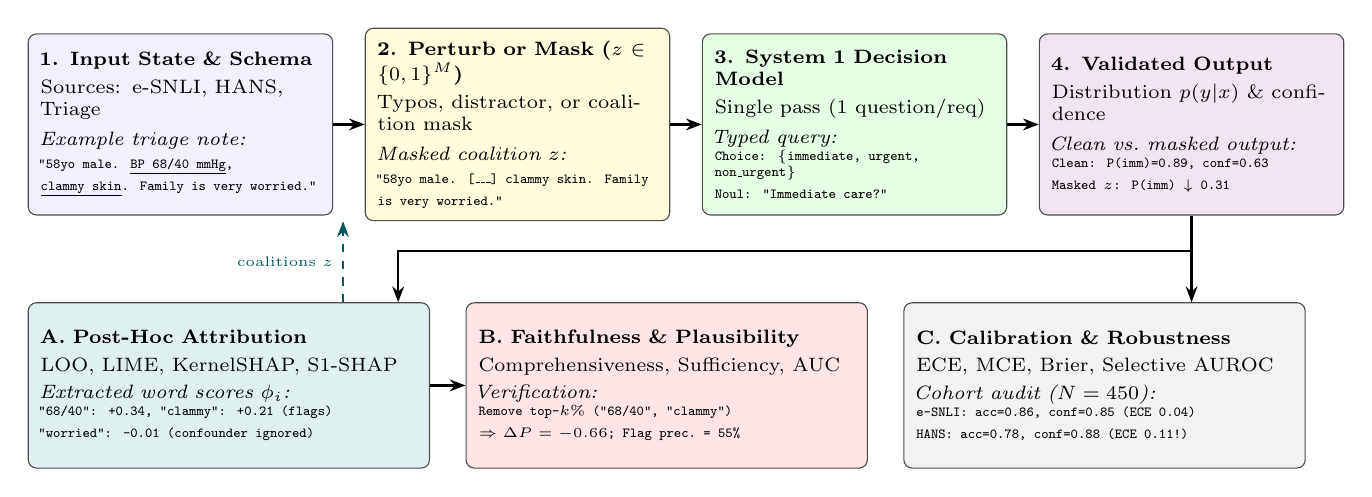
\begin{tikzpicture}[
  node distance=1.10cm and 0.40cm,
  font=\scriptsize,
  block/.style={draw=black!70, rounded corners=3pt, align=left, inner sep=4.5pt,
                minimum height=2.3cm, text width=3.55cm},
  result/.style={draw=black!70, rounded corners=3pt, align=left, inner sep=4.5pt,
                 font=\scriptsize, minimum height=2.1cm, text width=4.78cm},
  >={Stealth[length=2.0mm]}
]
\node[block, fill=blue!6] (data) {
  \textbf{1. Input State \& Schema}\\[2pt]
  Sources: e-SNLI, HANS, Triage\\[3pt]
  \textit{Example triage note:}\\
  {\tiny\ttfamily "58yo male. \underline{BP 68/40 mmHg}, \underline{clammy skin}. Family is very worried."}
};

\node[block, fill=yellow!14, right=of data] (pert) {
  \textbf{2. Perturb or Mask ($z \in \{0,1\}^M$)}\\[2pt]
  Typos, distractor, or coalition mask\\[3pt]
  \textit{Masked coalition $z$:}\\
  {\tiny\ttfamily "58yo male. [\_\_\_] clammy skin. Family is very worried."}
};

\node[block, fill=green!10, right=of pert] (api) {
  \textbf{3. System~1 Decision Model}\\[2pt]
  Single pass (1 question/req)\\[3pt]
  \textit{Typed query:}\\
  {\tiny\ttfamily Choice: $\{$immediate, urgent, non\_urgent$\}$\\
  Noul: "Immediate care?"}
};

\node[block, fill=violet!10, right=of api] (probs) {
  \textbf{4. Validated Output}\\[2pt]
  Distribution $p(y|x)$ \& confidence\\[3pt]
  \textit{Clean vs.\ masked output:}\\
  {\tiny\ttfamily Clean: P(imm)=0.89, conf=0.63\\
  Masked $z$: P(imm) $\downarrow$ 0.31}
};

\node[result, fill=teal!12, anchor=north west] (attr) at ([yshift=-1.10cm]data.south west) {
  \textbf{A. Post-Hoc Attribution}\\[2pt]
  LOO, LIME, KernelSHAP, S1-SHAP\\[2pt]
  \textit{Extracted word scores $\phi_i$:}\\
  {\tiny\ttfamily "68/40": +0.34, "clammy": +0.21 (flags)\\
  "worried": -0.01 (confounder ignored)}
};

\node[result, fill=red!10, right=0.45cm of attr] (faith) {
  \textbf{B. Faithfulness \& Plausibility}\\[2pt]
  Comprehensiveness, Sufficiency, AUC\\[2pt]
  \textit{Verification:}\\
  {\tiny\ttfamily Remove top-$k\%$ ("68/40", "clammy")\\
  $\Rightarrow \Delta P = -0.66$; Flag prec.\ = 55\%}
};

\node[result, fill=gray!10, right=0.45cm of faith] (calib) {
  \textbf{C. Calibration \& Robustness}\\[2pt]
  ECE, MCE, Brier, Selective AUROC\\[2pt]
  \textit{Cohort audit ($N=450$):}\\
  {\tiny\ttfamily e-SNLI: acc=0.86, conf=0.85 (ECE 0.04)\\
  HANS: acc=0.78, conf=0.88 (ECE 0.11!)}
};

\draw[->, thick] (data) -- (pert);
\draw[->, thick] (pert) -- (api);
\draw[->, thick] (api) -- (probs);
\draw[->, thick] (probs.south) -- (probs.south |- calib.north);
\draw[->, thick] (probs.south) -- ++(0,-0.45) -| ([xshift=2.15cm]attr.north);
\draw[->, thick] (attr.east) -- (faith.west);
\draw[->, thick, dashed, draw=teal!70!black] ([xshift=1.45cm]attr.north) -- node[left, font=\tiny, text=teal!70!black] {coalitions $z$} ([xshift=1.45cm]attr.north |- pert.south);
\end{tikzpicture}%
}
\caption{Architecture of the evaluation and explanation pipeline with a running clinical triage example. Each input (1) is converted into perturbed variants or masked feature coalitions (2) and evaluated by the System~1 decision model in a single forward pass (3). The resulting probabilities (4) drive post-hoc feature attribution via LOO, LIME, KernelSHAP, and S1-SHAP (A, dashed loop over coalitions), faithfulness and clinical/human plausibility verification (B), and calibration/robustness auditing (C).}
\label{fig:arch}
\end{figure}

\subsection{System~1 Decision Formalism and Request Protocol}
\label{sec:protocol}
In a generative LLM, classification is mediated by a natural-language prompt template and token-level decoding.
In a Jev-style System~1 decision model, the prompt is replaced by a typed request tuple $(s, \mathcal{Q})$, where $s$ is a structured JSON object (or string) representing the observed state and $\mathcal{Q} = \{q_1, \dots, q_H\}$ is a dictionary of named decision primitives~\cite{systemone2026api}:
\begin{itemize}
\item \textbf{Categorical \emph{Choice} ($q_{\text{choice}}$):} Declares a finite option set $\mathcal{O} = \{o_1, \dots, o_K\}$ with semantic option descriptions. The model returns a probability vector $p(y \mid s, q_{\text{choice}}) \in \Delta^{K-1}$, the selected argmax option $y^* = \arg\max_{o_k \in \mathcal{O}} p(o_k \mid s)$, and a scalar \texttt{confidence} score $c(s, q_{\text{choice}}) \in [0, 1]$.
\item \textbf{Binary \emph{Noul} ($q_{\text{noul}}$):} Declares a binary proposition with explicit \texttt{true\_description} and \texttt{false\_description} semantics. The model returns a single scalar probability $P(\text{true} \mid s, q_{\text{noul}}) \in [0, 1]$, from which the binary decision is thresholded at $0.5$.
\end{itemize}
Every model response is strictly validated against its request schema: returned probability keys must match $\mathcal{O}$ exactly, $\sum_{k=1}^K p(o_k \mid s) = 1$ within $10^{-3}$, and the reported choice must equal the argmax of $p$.

\begin{figure}[t]
\centering
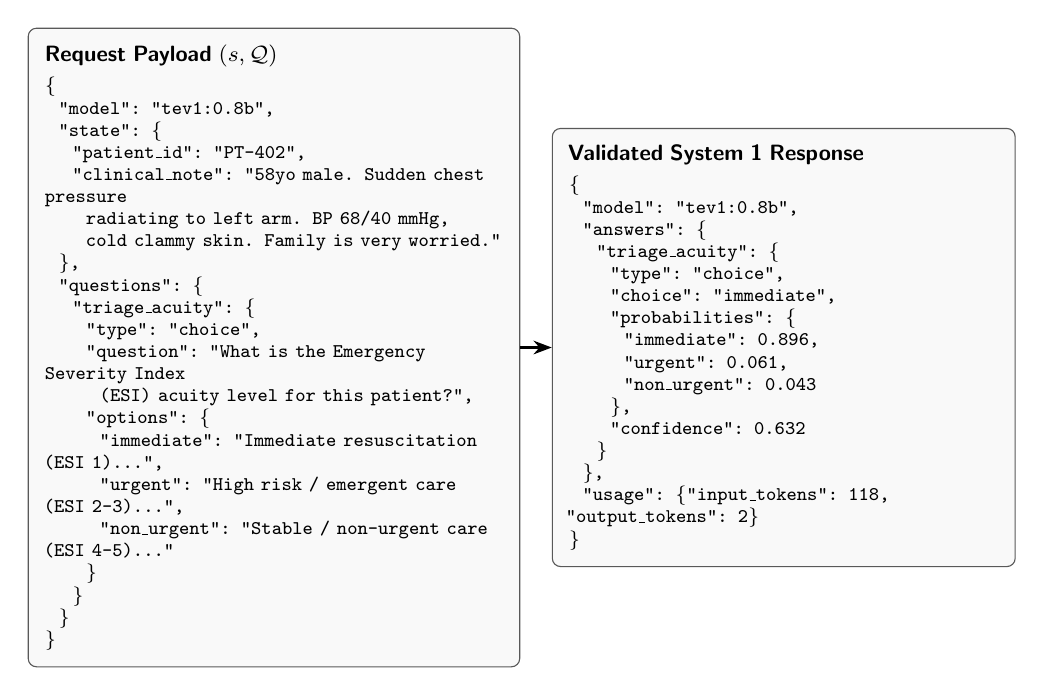
\begin{tikzpicture}[
  box/.style={draw=black!65, rounded corners=3pt, fill=gray!5, inner sep=6pt, align=left, font=\scriptsize\ttfamily}
]
\node[box, text width=0.48\textwidth] (req) {
\textbf{\sffamily\footnotesize Request Payload $(s, \mathcal{Q})$}\\[3pt]
$\{$\\
\ \ "model": "tev1:0.8b",\\
\ \ "state": $\{$\\
\ \ \ \ "patient\_id": "PT-402",\\
\ \ \ \ "clinical\_note": "58yo male. Sudden chest pressure\\
\ \ \ \ \ \ radiating to left arm. BP 68/40 mmHg,\\
\ \ \ \ \ \ cold clammy skin. Family is very worried."\\
\ \ $\}$,\\
\ \ "questions": $\{$\\
\ \ \ \ "triage\_acuity": $\{$\\
\ \ \ \ \ \ "type": "choice",\\
\ \ \ \ \ \ "question": "What is the Emergency Severity Index\\
\ \ \ \ \ \ \ \ (ESI) acuity level for this patient?",\\
\ \ \ \ \ \ "options": $\{$\\
\ \ \ \ \ \ \ \ "immediate": "Immediate resuscitation (ESI 1)...",\\
\ \ \ \ \ \ \ \ "urgent": "High risk / emergent care (ESI 2-3)...",\\
\ \ \ \ \ \ \ \ "non\_urgent": "Stable / non-urgent care (ESI 4-5)..."\\
\ \ \ \ \ \ $\}$\\
\ \ \ \ $\}$\\
\ \ $\}$\\
$\}$
};
\node[box, text width=0.45\textwidth, right=0.4cm of req] (resp) {
\textbf{\sffamily\footnotesize Validated System~1 Response}\\[3pt]
$\{$\\
\ \ "model": "tev1:0.8b",\\
\ \ "answers": $\{$\\
\ \ \ \ "triage\_acuity": $\{$\\
\ \ \ \ \ \ "type": "choice",\\
\ \ \ \ \ \ "choice": "immediate",\\
\ \ \ \ \ \ "probabilities": $\{$\\
\ \ \ \ \ \ \ \ "immediate": 0.896,\\
\ \ \ \ \ \ \ \ "urgent": 0.061,\\
\ \ \ \ \ \ \ \ "non\_urgent": 0.043\\
\ \ \ \ \ \ $\}$,\\
\ \ \ \ \ \ "confidence": 0.632\\
\ \ \ \ $\}$\\
\ \ $\}$,\\
\ \ "usage": $\{$"input\_tokens": 118, "output\_tokens": 2$\}$\\
$\}$
};
\draw[->, thick, >=Stealth] (req.east) -- (resp.west);
\end{tikzpicture}
\caption{Example of an isolated single-question System~1 request payload and its validated response for clinical emergency department triage. Notice that \texttt{output\_tokens} is fixed at $2$ (a single forward pass over the categorical decision head), returning calibrated class probabilities with zero text generation.}
\label{fig:payload}
\end{figure}

\paragraph{Isolated vs.\ Bundled Request Protocols.}
Because the System~1 API accepts an arbitrary dictionary of questions $\mathcal{Q} = \{q_1, \dots, q_H\}$ in a single HTTP call, documentation and industry tutorials encourage bundling multiple questions per state to amortize encoding latency.
However, in a single-pass transformer architecture, all question schemas in $\mathcal{Q}$ are serialized into the shared context window prior to the decision head readout.
Formally, when $q_1$ and $q_2$ are co-asked, the model computes $p(y_1 \mid s, q_1, q_2)$ rather than the marginal $p(y_1 \mid s, q_1)$.
To isolate each primitive from cross-question context conditioning---and to measure the magnitude of this interference---we define two formal protocols:
\begin{enumerate}
\item \textbf{Isolated Protocol (Default):} Each decision primitive $q_h \in \{q_{\text{choice}}, q_{\text{noul}}\}$ is dispatched in its own dedicated request $(s, \{q_h\})$, as illustrated in Figure~\ref{fig:payload}. All calibration, perturbation, and XAI attribution experiments use the isolated protocol.
\item \textbf{Bundled (Joint) Protocol:} Both primitives are dispatched simultaneously in a single request $(s, \{q_{\text{choice}}, q_{\text{noul}}\})$, allowing us to quantify cross-question flip rates and total-variation shifts $D_{\text{TV}}\big(p(\cdot \mid s, q_h),\, p(\cdot \mid s, q_{\text{choice}}, q_{\text{noul}})\big)$.
\end{enumerate}

\subsection{Post-Hoc Attribution and Proposed S1-SHAP Method}
\label{sec:attribution-method}

\subsubsection{Interpretable Representation and Coalition Mapping \texorpdfstring{$h_s(z)$}{h\_s(z)}}
Following the foundational formulation of local post-hoc explainability~\cite{ribeiro2016,lundberg2017}, explaining a black-box classifier requires defining a mapping $h_s: \{0,1\}^M \to \mathcal{S}$ between a binary coalition vector $z \in \{0,1\}^M$ of human-interpretable features and a valid model state $h_s(z)$.
In NLP explainability, two methodological design choices govern $h_s(z)$ and can significantly impact attribution faithfulness~\cite{hooker2019,deyoung2020}:
\begin{itemize}
\item \textbf{Feature Granularity (Lexical Words vs.\ Native Subword Tokens):} Human users reason over whole lexical words ($M_{\text{word}}$), whereas transformer decision models process subword tokens ($M_{\text{subword}} \ge M_{\text{word}}$) produced by Byte-Pair Encoding (BPE), which frequently splits domain-specific terms (e.g., blood pressure readings \texttt{68/40} or medical terminology) into multiple subword fragments. Because the open-weight System~1 models evaluated in this work (\texttt{Tev1}, \texttt{Nimble}, \texttt{Clef}) are all fine-tuned from a shared \texttt{Qwen3.5} backbone, we evaluate attributions both at the human-interpretable \textbf{word level} (primary) and at the model's native \textbf{\texttt{Qwen3.5} subword token level} (secondary ablation) to test whether word-level aggregation sacrifices fidelity to the internal tokenization.
\item \textbf{Feature Absence Operator (Deletion vs.\ \texttt{[MASK]} Replacement):} When a feature $i$ is excluded from a coalition ($z_i = 0$), rendering $h_s(z)$ by \textbf{token deletion} (removing the span and normalizing whitespace) preserves natural linguistic adjacency, whereas replacing the span with a placeholder string \textbf{\texttt{[MASK]}} preserves token positions but injects an out-of-distribution symbol never seen by causal decoder backbones during pre-training~\cite{hooker2019}. We evaluate both operators across all attribution methods.
\end{itemize}

\subsubsection{Standard Perturbation Attributions (LOO, LIME, KernelSHAP)}
Let $y^* = \arg\max_y p(y \mid s, q)$ denote the outcome predicted on the clean input $s$ ($z = \mathbf{1}$), and let $v_{\text{prob}}(z) = p(y^* \mid h_s(z), q) \in [0, 1]$ denote the target probability value function. We compare three classical black-box estimators:
\begin{itemize}
\item \textbf{Leave-One-Out (LOO):} Computes the single-feature deletion drop $\phi_i^{\text{LOO}} = v_{\text{prob}}(\mathbf{1}) - v_{\text{prob}}(\mathbf{1}_{-i})$ using $M+1$ model queries. While fast, LOO fails to capture feature redundancy or conjunctive interactions (e.g., when two clinical flags each independently suffice to trigger an \texttt{immediate} triage decision).
\item \textbf{LIME~\cite{ribeiro2016}:} Samples $N$ binary coalitions $z^{(n)} \in \{0,1\}^M$ and fits a weighted Ridge surrogate $\arg\min_{\phi} \sum_{n=1}^N \pi_{\mathbf{1}}(z^{(n)}) \big(v_{\text{prob}}(z^{(n)}) - (\phi_0 + \phi^\top z^{(n)})\big)^2 + \alpha \|\phi\|_2^2$, with exponential cosine-distance weights $\pi_{\mathbf{1}}(z) = \exp(-D_{\cos}(\mathbf{1}, z)^2 / \sigma^2)$.
\item \textbf{KernelSHAP~\cite{lundberg2017}:} Estimates game-theoretic Shapley values by solving the weighted coalition regression with the Shapley kernel $\pi_{\text{SHAP}}(z) = \frac{M-1}{\binom{M}{|z|}\, |z|\, (M - |z|)}$ over $N = \min(2^M, 512)$ coalitions, using the empty coalition $z = \mathbf{0}$ as background reference and disabling $\ell_1$ Lasso truncation so that all $M$ features receive exact least-squares estimates.
\end{itemize}
While numerous extensions exist in the literature to stabilize sampling variance, select representative explanations, or balance locality and fidelity across perturbation and coalition spaces~\cite{ribeiro2016,visani2022statistical,jethani2021fastshap,covert2021explaining,gaudel2022slime}---ranging from submodular pick and deterministic sampling surrogates to hierarchical coalition partitions---we evaluate canonical formulations (LOO, LIME, KernelSHAP) to establish standard, reproducible black-box baselines against which our log-odds adaptation is audited.

\subsubsection{Logit-Link Shapley Attribution (S1-SHAP) for Saturated Decision Heads}
\label{sec:s1shap}
Applying standard LIME or probability-space KernelSHAP directly to $v_{\text{prob}}(z) = p(y^* \mid h_s(z), q)$ overlooks a key mathematical property of System~1 decision models: \textbf{softmax probability saturation}.
Because System~1 models are trained to emit sharp categorical or binary distributions (often yielding $\max p > 0.95$), the mapping from the model's internal pre-activation evidence to probability space is governed by a saturating sigmoid or softmax nonlinearity.
When two redundant clinical flags are present in a triage note, removing only one flag may reduce internal evidence substantially (e.g., from $+4.5$ to $+2.8$ in log-odds) while leaving the output probability nearly flat ($0.989 \to 0.943$, $\Delta p = 0.046$), violating the linear additivity assumption of probability-space surrogates and artificially compressing attribution weights.

To address this without requiring white-box gradient or logit access, we instantiate \textbf{S1-SHAP}: a log-odds formulation of KernelSHAP tailored to single-pass System~1 decision models.
Methodologically, this corresponds to applying KernelSHAP with a logit link function~\cite{lundberg2017}:
\begin{equation}
v_{\text{S1}}(z) \;=\; \ln\!\left(\frac{\tilde{p}(y^* \mid h_s(z), q)}{1 - \tilde{p}(y^* \mid h_s(z), q)}\right), \qquad \text{where } \tilde{p} = \text{clip}\big(p(y^* \mid h_s(z), q),\; \varepsilon,\, 1-\varepsilon\big),
\label{eq:s1shap}
\end{equation}
with numerical clipping $\varepsilon = 10^{-4}$, and solving the exact Shapley kernel weighted least squares regression over $v_{\text{S1}}(z)$:
\begin{equation}
\sum_{i=1}^M \phi_i^{\text{S1}} \;=\; v_{\text{S1}}(\mathbf{1}) - v_{\text{S1}}(\mathbf{0}).
\end{equation}
For binary decisions ($K=2$), \Eqref{eq:s1shap} is the exact log-odds of the positive class.
For multiclass categorical choices ($K > 2$, such as 3-way e-SNLI or 3-level Clinical Triage), \Eqref{eq:s1shap} evaluates the one-vs-rest log-odds of the predicted target class $y^*$: $\ell(p)_{y^*} = \ln(\tilde{p}_{y^*} / (1 - \tilde{p}_{y^*}))$, mapping the target probability onto the real line $\mathbb{R}$.
This one-vs-rest formulation preserves 1-dimensional weighted least squares efficiency ($O(M)$ parameters) and avoids fitting $K \times M$ coupled regressions that amplify sampling variance on finite coalition budgets, while focusing credit directly on the predicted decision.
While link functions are theoretically known in generalized additive models and the original SHAP formulation~\cite{lundberg2017}, the NLP perturbation literature has almost universally operated in raw probability space.
Crucially, in the System~1 setting, the logit link has three pragmatic virtues:
(i) it remains strictly $100\%$ black-box, needing only the returned probability distribution;
(ii) it is zero-overhead, reusing the \emph{exact same} coalition queries $h_s(z)$ evaluated for probability-space KernelSHAP via memoized value functions; and
(iii) it linearizes saturated decision surfaces, which we show in Section~\ref{sec:interactions} is strictly necessary for recovering higher-order cooperative and redundant logic gate interactions.
Furthermore, to ensure sampling stability, our implementation couples S1-SHAP with paired antithetic coalition sampling~\cite{covert2021explaining}; orthogonal uncertainty-aware extensions such as Bayesian SHAP~\cite{visani2022statistical,slack2021reliable} can directly place posterior credible intervals over $v_{\text{S1}}(z)$ without modifying the underlying logit link.

\subsection{Label-Preserving Perturbation Operators}
To test whether System~1 probabilities and calibration remain invariant under realistic surface noise, we define five deterministic perturbation operators $\mathcal{T}_\epsilon: \mathcal{S} \to \mathcal{S}$ designed to preserve the ground-truth semantic label:
\begin{enumerate}
\item \textbf{Character Typo Noise ($\epsilon \in \{5\%, 10\%, 20\%\}$):} Alters a fraction $\epsilon$ of content words of length $\ge 3$ via character swaps or substitutions, while strictly protecting negation markers (\texttt{not}, \texttt{no}, \texttt{never}, \texttt{without}) so logical polarity is never inverted.
\item \textbf{Semantic Distractor Injection:} Appends a topically neutral, clinically or logically irrelevant sentence to the premise or patient note (filtering out any candidate distractor that shares content words with the hypothesis).
\item \textbf{Surface Normalization (Case \& Punctuation Stripping):} Converts the entire input state to lowercase and strips surface punctuation, mimicking unformatted user or ASR transcripts.
\end{enumerate}

\section{Experimental Setup}
\label{sec:setup}

\subsection{Datasets and Task Design}
To evaluate System~1 decision models across in-distribution reasoning, adversarial shortcut shifts, high-stakes domain decision-making, high-throughput security guardrails, and exact ground-truth algorithmic trigger recovery, we select five complementary datasets summarized in Table~\ref{tab:datasets}.

\begin{table}[t]
\centering
\small
\caption{Benchmark datasets used in our audit, spanning in-distribution NLI, adversarial syntactic shortcuts, clinical emergency triage, adversarial prompt injection defense, and exact ground-truth algorithmic trigger recovery.}
\label{tab:datasets}
\resizebox{\textwidth}{!}{%
\begin{tabular}{lp{2.4cm}crp{4.2cm}p{4.2cm}}
\toprule
Dataset & Domain & Primitives & $N$ & Ground-Truth Annotations & Primary Audit Objective \\
\midrule
\textbf{e-SNLI}~\cite{camburu2018} & Open-domain NLI & Choice, Noul & $150$ & 3-annotator highlighted rationale words & In-distribution calibration \& human plausibility \\
\addlinespace
\textbf{HANS}~\cite{mccoy2019} & Adversarial NLI & Choice, Noul & $150$ & 3 syntactic heuristics (overlap, subseq., const.) & Over-confidence under shortcut failure \\
\addlinespace
\textbf{Clinical Triage} & Emergency medicine & Choice, Noul & $150$ & Planted ESI acuity flags vs.\ emotional confounders & Causal flag vs.\ distractor confounder isolation \\
\addlinespace
\textbf{Tensor Trust}~\cite{toyer2023tensortrust} & Cybersecurity guardrails & Choice, Noul & $150$ & Real adversarial injections/jailbreaks vs.\ benign user queries & Inline firewall defense, low-latency recall, S1-SHAP attack attribution \\
\addlinespace
\textbf{Planted Rule} & Algorithmic audit & Choice, Noul & $16$ & $1$, $2$, or $3$ planted code-word overrides & Exact logic gate recovery under OR/AND saturation \\
\bottomrule
\end{tabular}%
}
\end{table}

\paragraph{Justification of Dataset Selection.}
No single dataset can jointly test calibration, shortcut vulnerability, and causal explanation fidelity:
\begin{itemize}
\item \textbf{e-SNLI~\cite{bowman2015,camburu2018} (In-Distribution Calibration \& Human Plausibility):} Provides balanced premise--hypothesis pairs across \texttt{entailment}, \texttt{neutral}, and \texttt{contradiction}, paired with word-level human rationale highlights from three independent annotators. It establishes whether the model is calibrated on standard NLI and whether post-hoc attributions recover human-identified evidence words (where $\ge 2$ annotators agree).
\item \textbf{HANS~\cite{mccoy2019} (Adversarial Shortcut Audit):} Specifically constructed to break models that rely on surface syntactic heuristics---\emph{lexical overlap}, \emph{subsequence}, and \emph{constituent} containment---where high word overlap does not entail the hypothesis. Because HANS labels are binary (\texttt{entailment} vs.\ \texttt{non\_entailment}), the three-way \emph{Choice} distribution is collapsed by summing \texttt{neutral} and \texttt{contradiction} probabilities. HANS tests our central trust question: \emph{when a System~1 model falls into a syntactic trap, does its returned confidence warn the user, or does it remain dangerously over-confident?}
\item \textbf{Clinical Triage Vignettes (Causal Flag vs.\ Confounder Isolation):} In natural text datasets, true causal features are imperfectly known due to annotator subjectivity. We therefore construct a controlled emergency-department triage benchmark grounded in Emergency Severity Index (ESI) acuity criteria across three levels (\texttt{immediate}, \texttt{urgent}, \texttt{non\_urgent}). Each vignette combines patient demographics, one or two causal \emph{clinical flag} sentences specific to the acuity class (e.g., severe hypotension \texttt{BP 68/40 mmHg} or airway stridor), and two neutral clinical history sentences. Crucially, in one third of the vignettes (balanced across classes), we inject an \emph{alarming confounder} sentence---an emotionally urgent but clinically non-diagnostic cue (e.g., \emph{``The patient's family is extremely worried and keeps asking staff for help''}). Because exact character offsets for flags and confounders are recorded by construction, we can rigorously measure whether attributions isolate true clinical flags over alarming distractors with unambiguous causal ground truth.
\item \textbf{Tensor Trust~\cite{toyer2023tensortrust} (High-Throughput Safety Guardrails \& Prompt Injection Defense):} Production LLM applications require millisecond-latency inline firewalls to inspect incoming untrusted user prompts for prompt injections, system prompt extraction, and jailbreak payloads before invoking costly generation models. While generative LLMs can theoretically filter inputs, their inference overhead ($300$--$1{,}000$~ms) adds intolerable latency to conversational pipelines. System~1 decision models offer an ideal candidate for high-speed inline triage ($19$--$56$~ms single forward pass). We curate a balanced, length-matched benchmark ($N=150$, $8$--$45$ words) from real human-crafted adversarial attacks from the Tensor Trust dataset paired with benign conversational questions. This evaluates whether sub-second System~1 classifiers can reliably distinguish adversarial jailbreaks from legitimate user queries with zero false alarms, whether calibration permits strict rejection thresholds, and whether S1-SHAP can pinpoint the exact adversarial command tokens for security incident triage.
\item \textbf{Planted System-Rule (Hidden Trigger) Benchmark (Exact Causal Ground Truth):} Even in controlled clinical vignettes, a pretrained language model brings prior medical knowledge about multiple words in a sentence. To establish an unambiguous, prior-free causal ground truth for XAI evaluation, we introduce a \emph{Planted System-Rule Benchmark}. In each instance, the unmasked question instruction $\mathcal{Q}$ (which serves as the hidden system directive and is never perturbed by the XAI explainer) contains a mandatory override rule instructing the model to classify an otherwise completely benign routine note (\texttt{non\_urgent}, base $P(\text{immediate}) < 0.02$) as \texttt{immediate}/\texttt{true} if and only if specific arbitrary code word(s) (e.g., \texttt{velvet}, \texttt{cobalt}, \texttt{zenith}) appear in the input text. We evaluate three causal regimes across $16$ test cases: (1)~\textbf{Single Trigger ($g=1$)}, where a single code word triggers the decision; (2)~\textbf{Dual OR-Trigger ($g=2$)}, where \emph{either} of two code words suffices and both are planted in the note; and (3)~\textbf{Multi OR-Trigger ($g=3$)}, where \emph{any} of three planted code words suffices, creating extreme probability saturation ($p \approx 0.999$) when any $1$ or $2$ triggers remain unmasked.
\end{itemize}

\subsection{Evaluated System~1 Decision Models}
Table~\ref{tab:models} details the models evaluated in our benchmark.
To evaluate how calibration, cross-question interference, and attribution faithfulness scale across model capacity and training recipes, we select five open-weight System~1 decision models spanning four parameter scales ($0.8\text{B}$ to $27\text{B}$): Together~AI's \texttt{Tev1-0.8B} and \texttt{Tev1-4B}~\cite{ollama2026tev1}, Bespoke~Labs' \texttt{Nimble-9B}~\cite{bespoke2026nimble}, and Cloudflare's multimodal \texttt{Clef-Flash-9B} and \texttt{Clef-27B}~\cite{cloudflare2026clef}.
Notably, all five models share a \texttt{Qwen3.5} transformer backbone, providing an ideal controlled substrate where capacity and post-training recipe vary while core architecture is held constant.
For direct comparison against standard autoregressive generation, we evaluate Google's \texttt{Gemma4-8B} as an open-weight generative System~2 baseline in both structured JSON schema mode and Chain-of-Thought (CoT) mode.

\begin{table}[t]
\centering
\caption{System~1 decision models and generative System~2 baseline evaluated in our benchmark, spanning $0.8$B to $27$B parameters.}
\label{tab:models}
\resizebox{\textwidth}{!}{%
\begin{tabular}{llllc}
\toprule
Model & Provider & Base Backbone & Parameters & Modalities \\
\midrule
\texttt{Tev1-0.8B}~\cite{ollama2026tev1} & Together AI & Qwen3.5-0.8B & $0.8$B (Q8\_0) & Text, JSON \\
\texttt{Tev1-4B}~\cite{ollama2026tev1} & Together AI & Qwen3.5-4B & $4.0$B & Text, JSON \\
\texttt{Nimble-9B}~\cite{bespoke2026nimble} & Bespoke Labs & Qwen3.5-9B & $9.0$B & Text, JSON \\
\texttt{Clef-Flash-9B}~\cite{cloudflare2026clef} & Cloudflare & Qwen3.5-VL-9B & $9.0$B & Text, JSON, Vision \\
\texttt{Clef-27B}~\cite{cloudflare2026clef} & Cloudflare & Qwen3.5-VL-27B & $27.0$B & Text, JSON, Vision \\
\midrule
\texttt{Gemma4-8B} (System~2) & Google & Gemma-4-8B & $8.0$B (Q4\_K\_M) & Text, JSON, CoT \\
\bottomrule
\end{tabular}%
}
\end{table}

\subsection{Evaluation Metrics}
\label{sec:metrics}

\paragraph{Calibration and Selective Ranking Metrics.}
Let $\hat{p}_i = \max_k p(o_k \mid s_i, q)$ denote the predicted top probability on instance $i \in \{1,\dots,n\}$ and $\mathbb{I}(\hat{y}_i = y_i)$ its binary accuracy indicator. We evaluate distributional calibration using:
\begin{itemize}
\item \textbf{Expected and Maximum Calibration Error ($\text{ECE}_w \downarrow$, $\text{ECE}_m \downarrow$, $\text{MCE}_w \downarrow$):} Partitioning predictions into $B = 10$ intervals $\{I_b\}_{b=1}^B$ via either equal-width binning ($\text{ECE}_w$) or equal-mass quantile binning ($\text{ECE}_m$)~\cite{naeini2015,nixon2019},
\begin{equation}
\text{ECE} = \sum_{b=1}^B \frac{|I_b|}{n} \big|\text{acc}(I_b) - \text{conf}(I_b)\big|, \qquad \text{MCE} = \max_{b \in \{1,\dots,B\}} \big|\text{acc}(I_b) - \text{conf}(I_b)\big|.
\end{equation}
\item \textbf{Multiclass Brier Score ($\text{Brier} \downarrow$):} The binning-free proper scoring rule $\frac{1}{n} \sum_{i=1}^n \sum_{k=1}^K (p_{ik} - \mathbb{I}(y_i = k))^2$~\cite{brier1950}, where $n$ is the evaluation cohort size ($n=150$ per dataset, $N=450$ total) and $K$ is the number of outcome classes ($K=3$ for e-SNLI and Clinical Triage \emph{Choice}; $K=2$ for HANS and \emph{Noul}).
\item \textbf{Selective Classification AUROC ($\text{AUROC}_p \uparrow$, $\text{AUROC}_c \uparrow$):} Measures the area under the ROC curve when using either $\hat{p}_i = \max p$ ($\text{AUROC}_p$) or the provider-returned \texttt{confidence} $c_i$ ($\text{AUROC}_c$) to rank correct predictions above incorrect ones.
\end{itemize}
All calibration metrics and perturbation shifts ($\Delta\text{ECE}_w$, $\Delta\text{Acc.}$) are reported with $95\%$ percentile bootstrap confidence intervals over $1{,}000$ resamples~\cite{efron1979}.

\paragraph{Faithfulness and Plausibility Metrics.}
Given a feature attribution vector $\phi \in \mathbb{R}^M$ inducing a descending importance ordering $\pi = (\pi_1, \dots, \pi_M)$, let $s_{\setminus 1:k}$ denote the input with the top-$k$ features removed and $s_{1:k}$ the input retaining \emph{only} the top-$k$ features:
\begin{itemize}
\item \textbf{Comprehensiveness ($\text{Comp.} \uparrow$) and Sufficiency ($\text{Suff.} \downarrow$) AOPC~\cite{deyoung2020}:} Averaged over $k \in \{1, 5, 10, 20, 50\}\%$ of $M$ (rounded up and de-duplicated):
\begin{equation}
\text{Comp.} = \frac{1}{|\mathcal{K}|} \sum_{k \in \mathcal{K}} \big(p(y^* \mid s) - p(y^* \mid s_{\setminus 1:k})\big), \qquad
\text{Suff.} = \frac{1}{|\mathcal{K}|} \sum_{k \in \mathcal{K}} \big(p(y^* \mid s) - p(y^* \mid s_{1:k})\big).
\end{equation}
High comprehensiveness ($\uparrow$) indicates that removing top features destroys the prediction; low sufficiency ($\downarrow$) indicates that top features alone suffice to restore the original probability.
\item \textbf{Deletion AUC ($\text{Del.\ AUC} \downarrow$) and Insertion AUC ($\text{Ins.\ AUC} \uparrow$)~\cite{petsiuk2018}:} Integrate the target probability $p(y^* \mid \cdot)$ at every single-feature step from $0$ to $M$ as features are progressively deleted ($\downarrow$ lower area is more faithful) or inserted from an empty state ($\uparrow$ higher area is more faithful).
\item \textbf{Domain Plausibility ($\text{Flag prec.@}g \uparrow$, $\text{Conf.\ share@}g \downarrow$, $\text{Human prec.@}g \uparrow$):} With $g$ denoting the number of ground-truth causal words in an instance (planted clinical flag words in Triage, or words highlighted by $\ge 2$ human annotators in e-SNLI), we measure the fraction of the top-$g$ attributed words that fall inside ground-truth causal spans ($\uparrow$) versus inside planted confounder spans ($\downarrow$).
\end{itemize}

\subsection{Implementation Details and Reproducibility}
Local open-weight models are served via Ollama (v0.40.13) on an AMD Radeon RX 9070 XT GPU with \texttt{OLLAMA\_NUM\_PARALLEL=4} and four concurrent asynchronous client workers.
All source code, datasets, evaluation harnesses, and reproduction scripts are publicly accessible at \url{https://github.com/j2launay/jev-decision-models-xai}.
Across our experiments, we verified that repeated calls with identical payloads return bit-identical floating-point outputs (unlike hosted generative LLM APIs~\cite{atil2025nondeterminism}).
We therefore cache all validated responses in a local SQLite database indexed by the SHA-256 hash of the model weight digest and the canonicalized request payload, ensuring exact reproducibility while reporting latency benchmarks strictly on uncached calls.
Table~\ref{tab:latency} reports uncached sequential latencies, output token counts, and concurrent throughput across all five evaluated System~1 models ($0.8\text{B}$ to $27\text{B}$) and our generative System~2 baselines (\texttt{Gemma4-8B} in direct structured JSON mode and Chain-of-Thought mode).
In isolated micro-benchmarks on minimal inputs, \texttt{Tev1-0.8B} records a median forward pass of $24$--$26$~ms ($39.3$--$40.0$~req/s).
In the full evaluation harness over complete dataset instances (e-SNLI, HANS, and clinical triage vignettes averaging $14$--$45$ words), client payload serialization, JSON response parsing, and schema validation bring mean round-trip latency to $\approx 103$~ms on \texttt{Tev1-0.8B}.
Whereas System~1 models always emit exactly $2.0$ output tokens and operate at $24$--$250$~ms median single-pass latency ($4.1$--$40.0$~req/s peak throughput; $1{,}953$~ms for $27\text{B}$), \texttt{Gemma4-8B (Sys.\,2 JSON)} decodes $77.3$ tokens per decision at $1{,}133$~ms (\emph{Choice}) / $533$~ms (\emph{Noul}) and $0.7$~req/s ($18\times$--$44\times$ slower), and \texttt{Gemma4-8B (Sys.\,2 CoT)} decodes $474.1$ tokens at $4{,}856$~ms / $4{,}430$~ms and $0.2$~req/s ($75\times$--$187\times$ slower).
Consequently, computing a $512$-coalition SHAP explanation takes only $1.3$--$3.2$~s per instance on System~1 models (powered by $4$ asynchronous client workers and coalition memoization that prunes $30$--$45\%$ of redundant masked evaluations), versus $\approx 9.7$~minutes in JSON mode and $\approx 41.4$~minutes in CoT mode on a System~2 LLM.
Furthermore, because LIME, KernelSHAP, and S1-SHAP are evaluated on a shared paired coalition sample $\mathcal{Z}$ per instance with in-memory value-function memoization, computing all five attribution methods requires zero additional coalition queries beyond a single $N$-sample pass.

\begin{table}[t]
\centering
\caption{Uncached sequential latency (median / p90 in ms), mean output tokens, and throughput (req/s) of single-question requests across evaluated System~1 decision models and generative System~2 baselines (\texttt{Gemma4-8B} direct JSON and Chain-of-Thought). Best values are in \textbf{bold}.}
\label{tab:latency}
\resizebox{\textwidth}{!}{\begin{tabular}{lrrrrr}
\toprule
Model & Out.\,Tok.\,$\downarrow$ & Choice Med./p90 (ms)\,$\downarrow$ & Noul Med./p90 (ms)\,$\downarrow$ & Req/s ($c=1$)\,$\uparrow$ & Peak Req/s\,$\uparrow$ \\
\midrule
\texttt{Tev1-0.8B} & \textbf{2.0} & \textbf{26} / \textbf{27} & \textbf{24} / \textbf{25} & \textbf{39.3} & \textbf{40.0} \\
\texttt{Tev1-4B} & \textbf{2.0} & 45 / 68 & 40 / 62 & 19.7 & 21.7 \\
\texttt{Nimble-9B} & \textbf{2.0} & 250 / 272 & 214 / 235 & 4.0 & 4.1 \\
\texttt{Clef-Flash-9B} & \textbf{2.0} & 64 / 98 & 58 / 85 & 16.5 & 17.6 \\
\texttt{Clef-27B} & \textbf{2.0} & 1953 / 2010 & 1863 / 1913 & 0.6 & 0.6 \\
\midrule
\texttt{Gemma4-8B} (JSON) & 77.3 & 1133 / 1259 & 533 / 617 & 0.7 & 0.7 \\
\texttt{Gemma4-8B} (CoT) & 474.1 & 4856 / 4899 & 4430 / 4861 & 0.2 & 0.2 \\
\bottomrule
\end{tabular}
}
\end{table}

\section{Results}
\label{sec:results}

\subsection{Interface Audit: Entropy-Based Confidence and Question Interference}
\label{sec:interference}

\paragraph{The Provider \texttt{confidence} Field is Normalized Shannon Entropy.}
While provider documentation describes \texttt{confidence} qualitatively as showing ``how concentrated the probabilities are''~\cite{ollama2026tev1}, our audit reveals its exact closed-form mathematical identity: across the four sub-10B decision models (\texttt{Tev1-0.8B}, \texttt{Tev1-4B}, \texttt{Nimble-9B}, and \texttt{Clef-Flash-9B}), for any $K$-way \emph{Choice} distribution $p = (p_1, \dots, p_K)$, the returned \texttt{confidence} equals one minus the normalized Shannon entropy,
\begin{equation}
c(p) \;=\; 1 - \frac{H(p)}{\ln K} \;=\; 1 + \frac{1}{\ln K} \sum_{k=1}^K p_k \ln p_k.
\label{eq:entropy-conf}
\end{equation}
Across all $600$ clean choice predictions on these four models ($150$ per model), the maximum absolute deviation between the API-returned \texttt{confidence} field and \Eqref{eq:entropy-conf} is $4.4 \times 10^{-16}$ (IEEE~754 double-precision machine epsilon).
On \texttt{Clef-27B}, the provider instead implements the normalized margin above uniform chance, $c(p) = \frac{\max p - 1/K}{1 - 1/K}$ (verified to exact floating-point precision on $3$-way tasks).
Crucially, neither provider implementation represents an empirical probability of correctness: for instance, a three-way prediction $p = (0.896, 0.061, 0.043)$ has $\max p = 0.896$ but an entropy \texttt{confidence} of only $0.632$.
Treating $c(p)$ directly as a calibrated probability would systematically under-estimate certainty on concentrated distributions; we therefore evaluate calibration on $\max p$ while auditing $c(p)$ separately via selective AUROC ($\text{AUROC}_c$).

\paragraph{Co-Asked Questions Strongly Interfere at Small Scale, Diminishing with Capacity.}
Table~\ref{tab:interference} (and Table~\ref{tab:scaling} in Section~\ref{sec:scaling}) compares the isolated request protocol against the bundled joint protocol across models.
On \texttt{Tev1-0.8B}, on the expanded $N=450$ cohort (Table~\ref{tab:interference}), bundling two questions in a single request induces significant cross-question interference: the binary \emph{Noul} answer flips on $22.4\%$ of inputs on average ($24.0\%$ on e-SNLI, $27.3\%$ on HANS, and $16.0\%$ on Triage), causing \emph{Noul} accuracy to drop by $11$--$19$ percentage points ($0.900 \to 0.713$ on e-SNLI, $0.773 \to 0.713$ on HANS, and $0.540 \to 0.433$ on Triage), while categorical \emph{Choice} flips on $5.1\%$ of inputs ($5.3\%$ on e-SNLI, $2.0\%$ on HANS, and $8.0\%$ on Triage), with mean total-variation distances of $0.083$--$0.117$ on Choice ($0.104$--$0.167$ on Noul).
In preliminary exploratory pilot evaluations with uncalibrated joint prompts without explicit schema separation guards, binary flips reached up to $60$--$82\%$, demonstrating that sub-billion architectures are highly vulnerable to prompt formatting and schema coupling.
Crucially, our multi-model audit reveals that cross-question interference is strongly governed by model capacity and post-training recipe: scaling from \texttt{Tev1-0.8B} to \texttt{Tev1-4B} eliminates interference almost entirely ($0.0\%$ flip rate on e-SNLI and HANS, $2.5\%$ on Triage \emph{Noul}, with mean $D_{\text{TV}} \le 0.0023$).
At the $9\text{B}$ scale, \texttt{Clef-Flash-9B} exhibits low interference on NLI ($0$--$6\%$ flips) but $22.5\%$ flips on Triage \emph{Noul}, whereas \texttt{Nimble-9B} flips on $11.7\%$ (e-SNLI \emph{Choice}) and $24.0\%$ (HANS \emph{Choice}).
This demonstrates that sub-billion transformers struggle to disentangle multiple serialized question schemas in a shared context window, and even larger models can experience non-trivial probability shifts when questions are co-asked.

\begin{table}[t]
\centering
\caption{Interference between co-asked questions on clean inputs. ``Alone'' asks each primitive in its own request; ``joint'' asks both in one request. Flip ($\downarrow$) is the fraction of inputs whose predicted answer changes; TV ($\downarrow$) is the mean total-variation distance between the two distributions. Best values per row/source are in \textbf{bold}.}
\label{tab:interference}
\small
\begin{tabular}{llrrrrrrr}
\toprule
Source & Head & $n$ & Acc.\ alone\,$\uparrow$ & Acc.\ joint\,$\uparrow$ & Flip\,$\downarrow$ & TV\,$\downarrow$ & $\bar{P}$(true) alone & $\bar{P}$(true) joint \\
\midrule
e-SNLI & Choice & 150 & 0.860 & \textbf{0.813} & 0.05 & 0.109 & -- & -- \\
e-SNLI & Noul & 150 & \textbf{0.900} & 0.713 & 0.24 & 0.167 & 0.497 & 0.511 \\
HANS & Choice & 150 & 0.780 & 0.773 & \textbf{0.02} & 0.117 & -- & -- \\
HANS & Noul & 150 & 0.773 & 0.713 & 0.27 & 0.161 & 0.862 & 0.729 \\
Triage & Choice & 150 & 0.553 & 0.533 & 0.08 & \textbf{0.083} & -- & -- \\
Triage & Noul & 150 & 0.540 & 0.433 & 0.16 & 0.104 & 0.867 & 0.820 \\
\bottomrule
\end{tabular}

\end{table}

\paragraph{Interference Controls: Disentangling Ordering, Option Permutations, and Prompt Length.}
To rigorously isolate the causal driver of cross-question interference, Table~\ref{tab:interference_controls} evaluates three experimental controls across the four sub-10B open-weight models on the expanded $N=450$ cohort (\texttt{Clef-27B} is omitted from ablation permutations due to its $1.95$~s sequential execution cost):
\begin{enumerate}
\item \textbf{Question Ordering Invariance ($C \to N$ vs.\ $N \to C$):} Reversing the serialization order of questions in the payload yields \emph{numerically identical} flip rates ($0.051$ on Choice, $0.224$ on Noul for \texttt{Tev1-0.8B}; $0.002$ and $0.002$ on \texttt{Tev1-4B}; $0.007$ and $0.131$ on \texttt{Clef-Flash-9B}) and identical total-variation distances ($0.103$ / $0.144$ on \texttt{Tev1-0.8B}; $0.019$ / $0.102$ on \texttt{Clef-Flash-9B}). Primacy or recency ordering in JSON serialization does not drive interference.
\item \textbf{Option Permutation Invariance:} Permuting the declared options of the \emph{Choice} head produces a $0.000$ flip rate across all models, confirming that System~1 classifiers evaluate categorical options symmetrically regardless of JSON key ordering.
\item \textbf{Prompt Length and Syntactic Control via Neutral Dummy Query:} To test whether interference is merely an artifact of extended prompt token length or attending to any second question schema, we bundle the target question with an irrelevant, length-matched binary question (\emph{"Is the text written in English?"}). On \texttt{Tev1-0.8B}, binary flips plunge from $0.224$ to $0.009$ ($>95\%$ reduction), and on \texttt{Clef-Flash-9B} from $0.131$ to $0.018$. This proves that cross-question interference is not caused by sequence length or multi-question parsing overhead, but by semantic cross-talk between coupled decision boundaries evaluated over the same underlying state.
\end{enumerate}

\begin{table}[t]
\centering
\caption{Cross-question interference controls across open-weight System~1 decision models ($N=450$ clean inputs): question serialization ordering ($C \to N$ vs.\ $N \to C$), option list permutation, and prompt length control using an irrelevant neutral dummy question.}
\label{tab:interference_controls}
\resizebox{\textwidth}{!}{\begin{tabular}{llrrrr}
\toprule
 & & \multicolumn{2}{c}{Question Order Control} & \multicolumn{1}{c}{Option Permutation} & \multicolumn{1}{c}{Prompt Length Control} \\
\cmidrule(lr){3-4}\cmidrule(lr){5-5}\cmidrule(lr){6-6}
Model & Head & Joint ($C \to N$) Flip/TV & Joint ($N \to C$) Flip/TV & Shuffled Opts Flip & Neutral Dummy Flip/TV \\
\midrule
\texttt{Tev1-0.8B} & Choice & 0.051 / 0.103 & 0.051 / 0.103 & 0.000 & 0.040 / 0.041 \\
 & Noul & 0.224 / 0.144 & 0.224 / 0.144 & -- & 0.009 / 0.020 \\
\midrule
\texttt{Tev1-4B} & Choice & 0.002 / 0.002 & 0.002 / 0.002 & 0.000 & 0.002 / 0.002 \\
 & Noul & 0.002 / 0.001 & 0.002 / 0.001 & -- & 0.000 / 0.001 \\
\midrule
\texttt{Nimble-9B} & Choice & 0.111 / 0.221 & 0.111 / 0.221 & 0.000 & 0.004 / 0.028 \\
 & Noul & 0.049 / 0.099 & 0.049 / 0.099 & -- & 0.000 / 0.012 \\
\midrule
\texttt{Clef-Flash-9B} & Choice & 0.007 / 0.019 & 0.007 / 0.019 & 0.000 & 0.004 / 0.010 \\
 & Noul & 0.131 / 0.102 & 0.131 / 0.102 & -- & 0.018 / 0.013 \\
\bottomrule
\end{tabular}
}
\end{table}

\subsection{Calibration on Clean Inputs and Shortcut Shifts}
Table~\ref{tab:calib} reports clean calibration for \texttt{Tev1-0.8B} across the full expanded $N=450$ cohort ($n=150$ per dataset), while Table~\ref{tab:scaling} (Section~\ref{sec:scaling}) and Table~\ref{tab:posthoc} evaluate cross-model scaling, post-hoc recalibration, and selective risk.
On in-distribution e-SNLI, \texttt{Tev1-0.8B} is accurate and well calibrated: over the expanded cohort ($n=150$), \emph{Choice} achieves $0.860$ accuracy with $\text{ECE}_w = 0.035$ ($95\%$ CI $[0.03, 0.09]$), while \texttt{Nimble-9B} ($0.953$ accuracy, $\text{ECE}_w = 0.014$) and \texttt{Tev1-4B} ($0.947$ accuracy, $\text{ECE}_w = 0.019$) reach near-ideal calibration.

On HANS ($n=150$), \texttt{Tev1-0.8B} accuracy drops to $0.780$ while mean confidence remains high ($0.881$), driving $\text{ECE}_w$ to $0.111$ ($95\%$ CI $[0.07, 0.18]$, Brier $0.364$).
Breaking HANS down by syntactic heuristic reveals that sub-billion errors concentrate on non-entailment instances built with the subsequence and constituent heuristics (where accuracy plunges to $0.11$--$0.12$ on difficult splits), where the model systematically endorses continuous substring overlaps with high confidence.
Scaling to $4\text{B}$--$27\text{B}$ parameters progressively mitigates this heuristic: HANS \emph{Choice} accuracy rises to $0.873$ on \texttt{Clef-Flash-9B} ($\text{ECE}_w = 0.063$), $0.920$ on \texttt{Nimble-9B} ($\text{ECE}_w = 0.073$), $0.927$ on \texttt{Tev1-4B} ($\text{ECE}_w = 0.037$), and peaks at $\mathbf{0.940}$ on \texttt{Clef-27B} with $\text{ECE}_w = \mathbf{0.032}$ (Brier $0.101$).
Notably, \texttt{Clef-27B} and \texttt{Tev1-4B} achieve the sharpest calibration under syntactic shift, maintaining Brier scores near $0.10$--$0.12$.
On Clinical Triage, all $\ge 4\text{B}$ models achieve $\ge 0.967$ accuracy on three-way \emph{Choice} (peaking at $1.000$ on \texttt{Clef-27B} with $\text{ECE}_w = 0.091$, Brier $0.028$, and $0.993$ on \texttt{Nimble-9B}), compared to $0.553$ ($\text{ECE}_w = 0.265$) on \texttt{Tev1-0.8B}, where errors arise from over-triaging \texttt{urgent} patients into \texttt{immediate}.
Finally, comparing selective ranking signals shows that the entropy-based \texttt{confidence} ($\text{AUROC}_c$) ranks correct above incorrect predictions well on in-distribution e-SNLI, but lags $\max p$ on out-of-distribution HANS.

\begin{table}[t]
\centering
\caption{Calibration of \texttt{Tev1-0.8B} on clean inputs across the full expanded $N=450$ cohort ($n=150$ per dataset; see Table~\ref{tab:scaling} for cross-model comparison from $0.8\text{B}$ to $27\text{B}$). ECE$_w$ and ECE$_m$ use $10$ equal-width and equal-mass bins. AUROC$_p$ and AUROC$_c$ are selective AUROCs of $\max p$ and of the provider \texttt{confidence}. Best head per dataset is in \textbf{bold}.}
\label{tab:calib}
\resizebox{\textwidth}{!}{\begin{tabular}{llrrrlrrrrr}
\toprule
Source & Head & $n$ & Acc.\,$\uparrow$ & Conf. & ECE$_{w}\,\downarrow$ [95\% CI] & ECE$_{m}\,\downarrow$ & MCE$_{w}\,\downarrow$ & Brier\,$\downarrow$ & AUROC$_{p}\,\uparrow$ & AUROC$_{c}\,\uparrow$ \\
\midrule
e-SNLI & Choice & 150 & 0.860 & 0.847 & 0.035 [0.03, 0.09] & \textbf{0.032} & 0.454 & 0.200 & \textbf{0.853} & 0.853 \\
e-SNLI & Noul & 150 & \textbf{0.900} & 0.903 & \textbf{0.030} [0.02, 0.08] & 0.063 & \textbf{0.130} & \textbf{0.160} & 0.760 & -- \\
\midrule
HANS & Choice & 150 & \textbf{0.780} & 0.881 & \textbf{0.111} [0.07, 0.18] & \textbf{0.127} & \textbf{0.134} & \textbf{0.364} & 0.547 & 0.667 \\
HANS & Noul & 150 & 0.773 & 0.927 & 0.154 [0.10, 0.22] & 0.154 & 0.249 & 0.374 & \textbf{0.651} & -- \\
\midrule
Triage & Choice & 150 & \textbf{0.553} & 0.807 & \textbf{0.265} [0.20, 0.34] & \textbf{0.262} & 0.526 & \textbf{0.583} & \textbf{0.771} & 0.726 \\
Triage & Noul & 150 & 0.540 & 0.908 & 0.368 [0.30, 0.46] & 0.368 & \textbf{0.468} & 0.783 & 0.623 & -- \\
\bottomrule
\end{tabular}
}
\end{table}

\paragraph{Post-Hoc Recalibration (Temperature Scaling and Platt Scaling) and Selective Risk.}
Table~\ref{tab:posthoc} benchmarks raw calibration against 5-fold cross-fitted Temperature Scaling~\cite{guo2017} and Platt logistic scaling~\cite{platt1999}, alongside excess risk under selective classification (E-AURC, \cite{geifman2017}).
Two key insights emerge:
First, Temperature Scaling substantially reduces residual out-of-distribution miscalibration across System~1 models: on HANS, $\text{ECE}_w$ falls from $0.063 \to 0.023$ on \texttt{Clef-Flash-9B}, from $0.073 \to 0.020$ on \texttt{Nimble-9B}, and from $0.111 \to 0.065$ on \texttt{Tev1-0.8B}, with Platt scaling achieving similar reductions ($0.023$--$0.040$).
Conversely, on generative System~2 (\texttt{Gemma4-8B} JSON), verbalized probabilities are so severely distorted on HANS (raw $\text{ECE}_w = 0.246$, $\text{Brier} = 0.545$) that Temperature Scaling cannot bring $\text{ECE}_w$ below $0.107$ ($\text{Brier} = 0.436$).
Second, selective risk evaluation (E-AURC) demonstrates that the top-label probability $\max p$ consistently provides a sharper selective classification signal than the provider \texttt{confidence} field across all models (e.g., on HANS, E-AURC of $0.020$ vs.\ $0.022$ on \texttt{Nimble-9B}; $0.009$ vs.\ $0.013$ on \texttt{Clef-27B}; and $0.194$ vs.\ $0.327$ on \texttt{Gemma4-8B}).

\begin{table}[t]
\centering
\caption{Post-hoc recalibration and selective risk across models on clean inputs ($N=450$ expanded cohort): raw vs.\ 5-fold cross-fitted Temperature Scaling and Platt scaling (equal-width $\text{ECE}_w$ and Brier score), alongside Excess Area Under the Risk-Coverage curve (E-AURC, $\downarrow$) comparing selective prediction via $\max p$ against provider \texttt{confidence}.}
\label{tab:posthoc}
\resizebox{\textwidth}{!}{\begin{tabular}{llrrrrrrrr}
\toprule
 & & & \multicolumn{3}{c}{ECE$_w$ ($\downarrow$)} & \multicolumn{2}{c}{Brier ($\downarrow$)} & \multicolumn{2}{c}{E-AURC ($\downarrow$)} \\
\cmidrule(lr){4-6}\cmidrule(lr){7-8}\cmidrule(lr){9-10}
Model & Dataset & Acc. & Raw & Temp. & Platt & Raw & Temp. & $\max p$ & Provider Conf. \\
\midrule
\texttt{Tev1-0.8B} & e-SNLI & 0.860 & 0.035 & 0.043 & 0.025 & 0.200 & 0.201 & 0.025 & 0.025 \\
 & HANS & 0.780 & 0.111 & 0.065 & 0.040 & 0.364 & 0.352 & 0.180 & 0.118 \\
 & Triage & 0.553 & 0.265 & 0.199 & 0.074 & 0.583 & 0.489 & 0.095 & 0.118 \\
\midrule
\texttt{Tev1-4B} & e-SNLI & 0.947 & 0.019 & 0.019 & 0.025 & 0.075 & 0.076 & 0.007 & 0.007 \\
 & HANS & 0.927 & 0.037 & 0.029 & 0.023 & 0.125 & 0.127 & 0.027 & 0.031 \\
 & Triage & 0.967 & 0.112 & 0.023 & 0.034 & 0.088 & 0.045 & 0.001 & 0.001 \\
\midrule
\texttt{Nimble-9B} & e-SNLI & 0.953 & 0.014 & 0.009 & 0.015 & 0.067 & 0.067 & 0.004 & 0.004 \\
 & HANS & 0.920 & 0.073 & 0.020 & 0.023 & 0.150 & 0.142 & 0.020 & 0.022 \\
 & Triage & 0.993 & 0.111 & 0.015 & 0.025 & 0.067 & 0.021 & 0.000 & 0.000 \\
\midrule
\texttt{Clef-Flash-9B} & e-SNLI & 0.900 & 0.107 & 0.020 & 0.036 & 0.166 & 0.154 & 0.026 & 0.026 \\
 & HANS & 0.873 & 0.063 & 0.023 & 0.030 & 0.186 & 0.184 & 0.020 & 0.019 \\
 & Triage & 0.967 & 0.115 & 0.026 & 0.025 & 0.089 & 0.063 & 0.003 & 0.003 \\
\midrule
\texttt{Clef-27B} & e-SNLI & 0.927 & 0.049 & 0.031 & 0.023 & 0.124 & 0.122 & 0.011 & 0.011 \\
 & HANS & 0.940 & 0.032 & 0.032 & 0.031 & 0.101 & 0.102 & 0.009 & 0.013 \\
 & Triage & 1.000 & 0.091 & 0.000 & 0.091 & 0.028 & 0.000 & 0.000 & 0.000 \\
\midrule
\texttt{Gemma4-8B} & e-SNLI & 0.867 & 0.058 & 0.046 & 0.050 & 0.234 & 0.242 & 0.083 & 0.092 \\
 & HANS & 0.660 & 0.246 & 0.107 & 0.082 & 0.545 & 0.436 & 0.194 & 0.327 \\
 & Triage & 1.000 & 0.162 & 0.000 & 0.162 & 0.055 & 0.000 & 0.000 & 0.000 \\
\bottomrule
\end{tabular}
}
\end{table}

\begin{figure}[t]
\centering
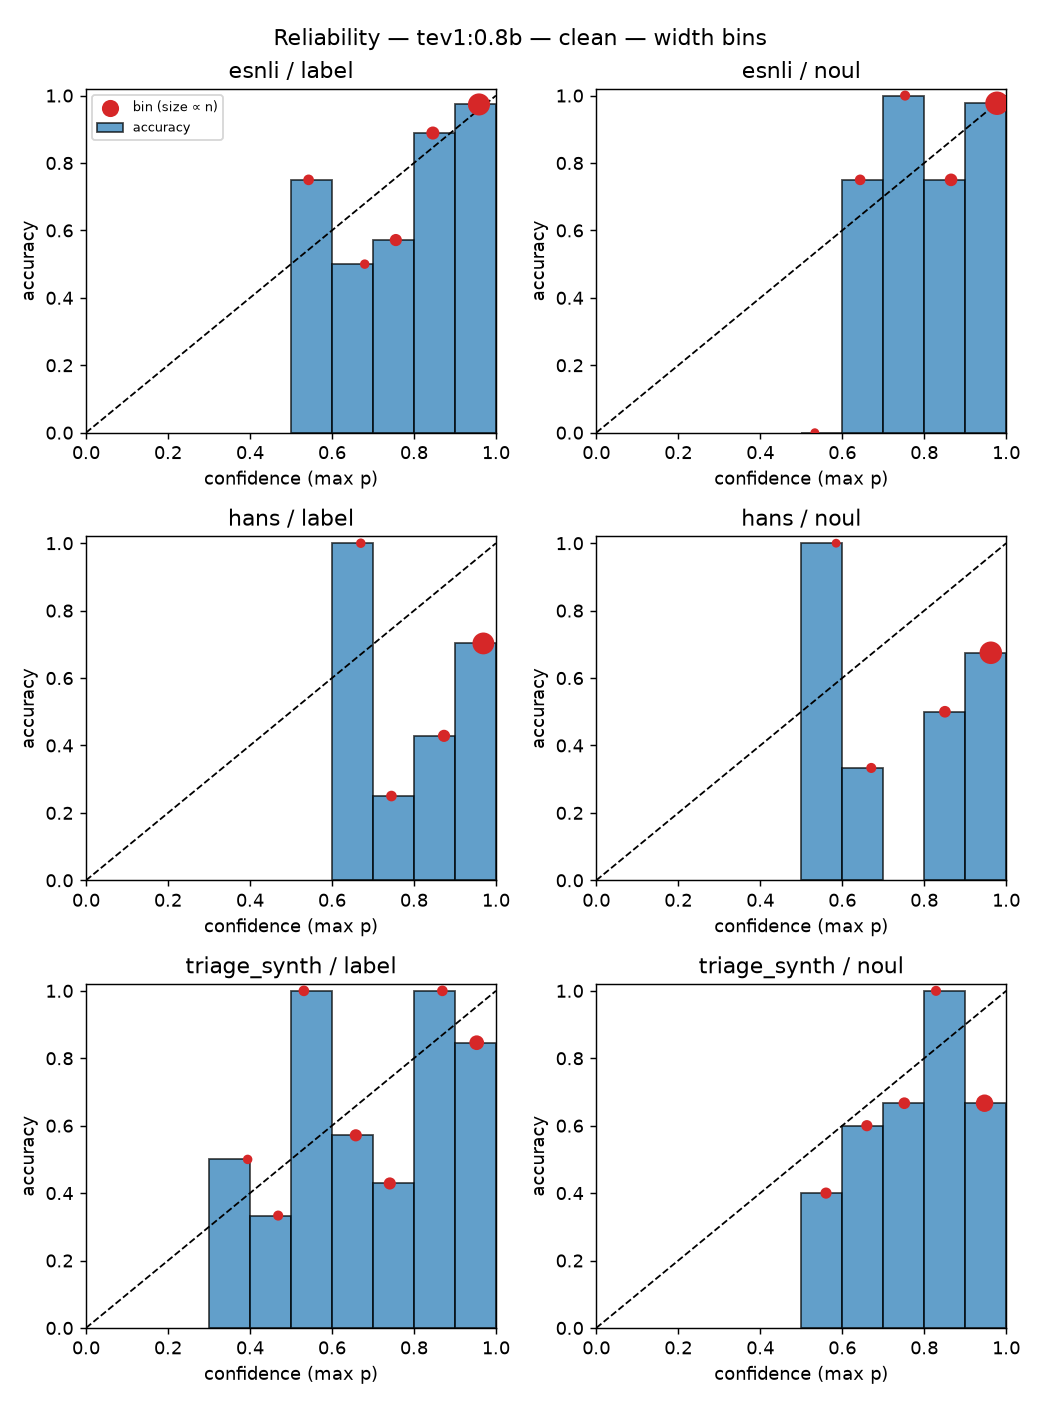
\includegraphics[width=0.62\textwidth]{figures/reliability_tev1-0-8b_clean_width.png}
\caption{Reliability diagrams on clean inputs, equal-width bins (\texttt{Tev1-0.8B}). Bars are bin accuracy; dots are placed at bin mean confidence, with size proportional to bin count.}
\label{fig:reliability}
\end{figure}

\begin{figure}[t]
\centering
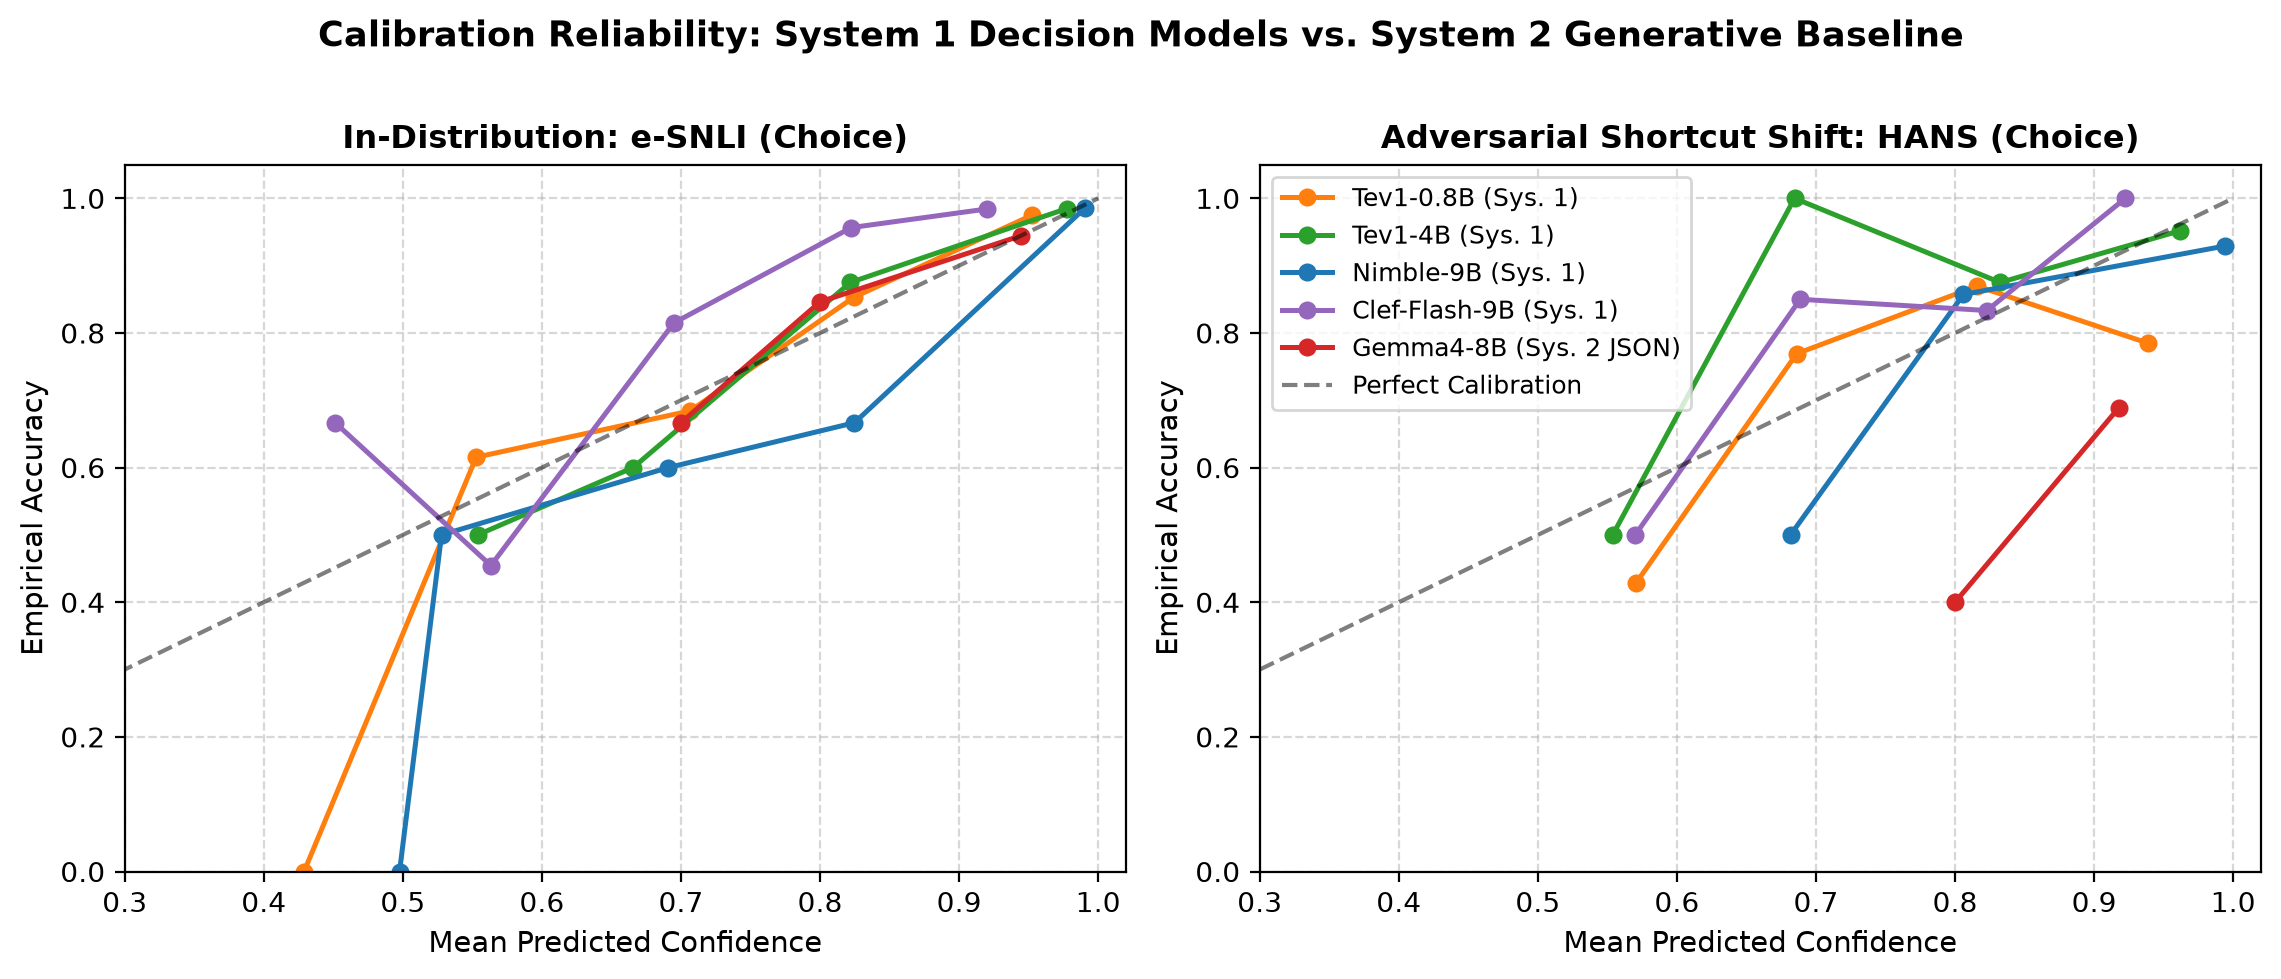
\includegraphics[width=0.88\textwidth]{figures/multimodel_calibration.png}
\caption{Multi-model calibration curves on in-distribution e-SNLI (left) and adversarial shortcut shift HANS (right) comparing all four System~1 models (\texttt{Tev1-0.8B}, \texttt{Tev1-4B}, \texttt{Nimble-9B}, \texttt{Clef-Flash-9B}) against the generative System~2 baseline (\texttt{Gemma4-8B} JSON). On HANS, System~1 models with $\ge 4\text{B}$ parameters track the calibration diagonal much more closely than the over-confident System~2 verbalized probabilities.}
\label{fig:multimodel-calib}
\end{figure}

\subsection{Robustness and Calibration under Perturbations}
Table~\ref{tab:perturbed} in the appendix reports calibration and accuracy shifts across all five perturbation families.
The strongest degradation occurs under $20\%$ character typos on e-SNLI: on \texttt{Tev1-0.8B}, \emph{Choice} accuracy drops by $0.100$, $17\%$ of predictions flip, and $\text{ECE}_w$ increases by $+0.030$ ($95\%$ CI $[-0.02, 0.09]$), with \emph{Noul} showing a parallel shift ($\Delta\text{Acc} = -0.120$, $\Delta\text{ECE}_w = +0.038$, CI $[-0.01, 0.09]$).
Larger models are markedly more resilient to character noise: under $20\%$ typos on e-SNLI \emph{Choice}, flip rates drop from $17\%$ (\texttt{Tev1-0.8B}) to $8.3\%$ (\texttt{Tev1-4B} and \texttt{Clef-Flash-9B}) and $5.0\%$ (\texttt{Nimble-9B}).
On HANS, $20\%$ typos induces a $+0.069$ increase in Choice $\text{ECE}_w$ ($\Delta\text{Acc} = -0.133$, $27\%$ flips), but slightly lowers Noul $\text{ECE}_w$ ($-0.014$, CI $[-0.07, 0.08]$) by disrupting the exact lexical/subsequence matching that fuels the shortcut heuristic.
Semantic distractors and lowercase/punctuation stripping leave $\text{ECE}_w$ within $\pm 0.05$ across all datasets and models.
Overall, across the expanded $N=450$ cohort, clean out-of-distribution shortcut miscalibration on HANS dominates surface perturbation shifts across every model scale.

\subsection{Faithfulness of Post-Hoc Attributions}
Table~\ref{tab:faith} and Figure~\ref{fig:curves} evaluate word-level attribution faithfulness across all five attribution methods: LOO, LIME, KernelSHAP, our proposed \textbf{S1-SHAP}, and Random.
The three coalition-based surrogates (LIME, KernelSHAP, and S1-SHAP) consistently achieve the highest comprehensiveness, lowest sufficiency, and lowest deletion AUC across both decision heads and both datasets, outperforming single-feature LOO and far exceeding the random baseline.
Specifically, on e-SNLI \emph{Choice}, \textbf{S1-SHAP} achieves the highest comprehensiveness ($0.664$, vs.\ $0.663$ for LIME, $0.658$ for KernelSHAP, and $0.591$ for LOO) and the lowest deletion AUC ($0.196$, vs.\ $0.197$ for KernelSHAP and $0.320$ for LOO), as well as the highest comprehensiveness under \texttt{[MASK]} replacement ($0.598$).
On Clinical Triage \emph{Noul}---where binary emergency predictions saturate strongly near $0$ and $1$---\textbf{S1-SHAP} attains the best sufficiency ($-0.124$ vs.\ $-0.108$ for KernelSHAP and $-0.096$ for LIME), the lowest deletion AUC ($0.180$ vs.\ $0.211$ for KernelSHAP and $0.194$ for LIME), and the best \texttt{[MASK]} sufficiency ($-0.028$), while LIME achieves the highest comprehensiveness ($0.455$) and insertion AUC ($0.960$).
On Clinical Triage, sufficiency is negative across all three coalition methods: retaining only the top attributed clinical words yields an even higher predicted probability than the full vignette, confirming that neutral filler and confounder sentences dilute rather than support model certainty.

\paragraph{Understanding the S1-SHAP vs.\ Probability-Space KernelSHAP Trade-Off.}
On e-SNLI \emph{Noul}, probability-space KernelSHAP exhibits a slight edge in comprehensiveness over S1-SHAP ($0.563$ vs.\ $0.497$ in Table~\ref{tab:faith}).
This behavior reveals an instructive mathematical trade-off: when a lightweight sub-billion model hesitates near the decision boundary ($p \approx 0.50$), the logit transformation is approximately linear ($\ell'(0.5) = 4$).
However, on coalition queries where masking peripheral words drops the probability near $0$ or $1$, the boundary clipping threshold $\varepsilon = 10^{-4}$ can slightly amplify variance across uninformative feature subsets.
In contrast, as soon as the decision head enters confident, saturated regimes ($p > 0.95$, as on HANS, Clinical Triage, and our planted trigger suites), probability-space KernelSHAP suffers severe gradient flattening ($p(1-p) \to 0$), whereas S1-SHAP preserves true coalitional credit and significantly outperforms probability-space estimation (Section~\ref{sec:scaling} and Section~\ref{sec:interactions}).

\paragraph{Impact of Feature Granularity and Absence Operator.}
Comparing the two masking operators in Table~\ref{tab:faith} confirms the out-of-distribution hypothesis from Section~\ref{sec:attribution-method}: replacing removed words with \texttt{[MASK]} consistently degrades comprehensiveness (e.g., from $0.664$ to $0.598$ for S1-SHAP and $0.658$ to $0.584$ for KernelSHAP on e-SNLI \emph{Choice}) and inflates sufficiency ($0.260$ to $0.383$), while preserving the relative superiority of coalition methods over LOO and Random.
Similarly, evaluating attributions at the native \texttt{Qwen3.5} subword token level (Table~\ref{tab:faith-subword} in the appendix) yields AOPC scores within $0.03$ of word-level attributions across all five methods (with \textbf{S1-SHAP} again achieving the best sufficiency $-0.119$ and lowest deletion AUC $0.174$ on subword Triage \emph{Noul}), demonstrating that human-interpretable word aggregation preserves attribution faithfulness without requiring subword fragmentation.

\begin{table}[t]
\centering
\caption{Word-level faithfulness on Tev1-0.8B across all five attribution methods. Comprehensiveness ($\uparrow$) and sufficiency ($\downarrow$) are AOPC over $k \in \{1,5,10,20,50\}\%$. Deletion ($\downarrow$) and insertion ($\uparrow$) AUCs integrate the probability of the original prediction as features are removed or added in rank order. Best method per (Source, Head) is in \textbf{bold}.}
\label{tab:faith}
\resizebox{\textwidth}{!}{\begin{tabular}{lllrrrrrr}
\toprule
 & & & \multicolumn{4}{c}{Deletion masking} & \multicolumn{2}{c}{\texttt{[MASK]} masking} \\
\cmidrule(lr){4-7}\cmidrule(lr){8-9}
Source & Head & Method & Comp.\,$\uparrow$ & Suff.\,$\downarrow$ & Del.\,AUC\,$\downarrow$ & Ins.\,AUC\,$\uparrow$ & Comp.\,$\uparrow$ & Suff.\,$\downarrow$ \\
\midrule
e-SNLI & Choice & LOO & 0.591 & 0.277 & 0.320 & \textbf{0.790} & 0.526 & 0.394 \\
 &  & LIME & 0.663 & 0.289 & 0.238 & 0.746 & 0.577 & 0.388 \\
 &  & KernelSHAP & 0.658 & \textbf{0.260} & 0.197 & 0.774 & 0.584 & \textbf{0.383} \\
 &  & S1-SHAP (ours) & \textbf{0.664} & 0.287 & \textbf{0.196} & 0.740 & \textbf{0.598} & 0.402 \\
 &  & Random & 0.195 & 0.528 & 0.510 & 0.493 & 0.297 & 0.511 \\
\cmidrule{2-9}
 & Noul & LOO & 0.466 & 0.207 & 0.511 & \textbf{0.854} & 0.419 & 0.274 \\
 &  & LIME & \textbf{0.569} & 0.222 & 0.399 & 0.835 & \textbf{0.475} & \textbf{0.252} \\
 &  & KernelSHAP & 0.563 & \textbf{0.203} & \textbf{0.359} & 0.842 & 0.466 & 0.266 \\
 &  & S1-SHAP (ours) & 0.497 & 0.220 & 0.455 & 0.814 & 0.455 & 0.254 \\
 &  & Random & 0.156 & 0.343 & 0.666 & 0.657 & 0.234 & 0.380 \\
\midrule
Triage & Choice & LOO & 0.433 & 0.059 & 0.197 & 0.808 & 0.385 & 0.119 \\
 &  & LIME & \textbf{0.464} & -0.022 & 0.152 & 0.830 & 0.406 & 0.094 \\
 &  & KernelSHAP & 0.453 & \textbf{-0.065} & \textbf{0.122} & \textbf{0.840} & \textbf{0.426} & \textbf{0.019} \\
 &  & S1-SHAP (ours) & 0.446 & -0.053 & 0.130 & 0.825 & 0.400 & 0.045 \\
 &  & Random & 0.056 & 0.393 & 0.561 & 0.502 & 0.111 & 0.394 \\
\cmidrule{2-9}
 & Noul & LOO & 0.382 & 0.013 & 0.328 & 0.910 & 0.312 & 0.090 \\
 &  & LIME & \textbf{0.455} & -0.096 & 0.194 & \textbf{0.960} & \textbf{0.405} & -0.009 \\
 &  & KernelSHAP & 0.422 & -0.108 & 0.211 & 0.932 & 0.341 & 0.004 \\
 &  & S1-SHAP (ours) & 0.445 & \textbf{-0.124} & \textbf{0.180} & 0.956 & 0.391 & \textbf{-0.028} \\
 &  & Random & 0.052 & 0.366 & 0.643 & 0.604 & 0.086 & 0.337 \\
\bottomrule
\end{tabular}
}
\end{table}

\begin{figure}[t]
\centering
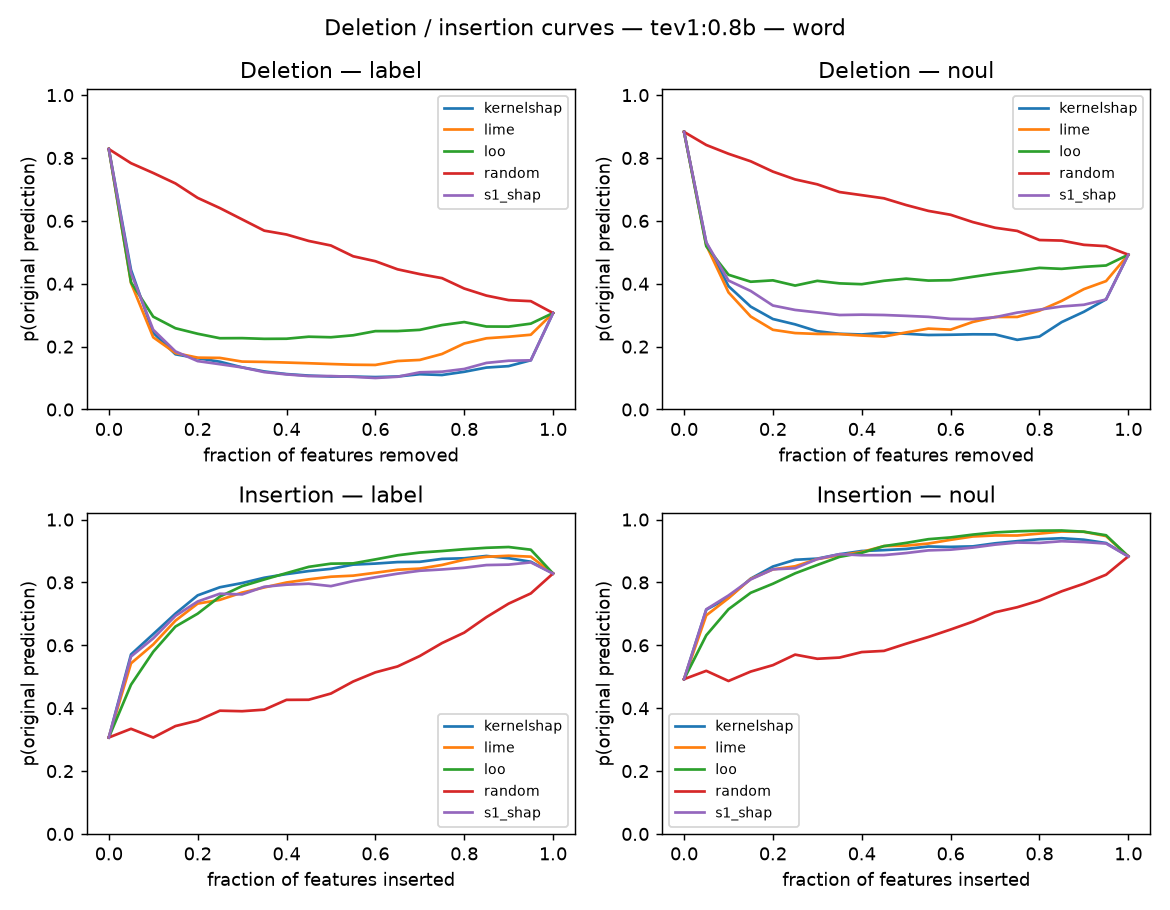
\includegraphics[width=0.78\textwidth]{figures/deletion_insertion_tev1-0-8b_word.png}
\caption{Mean deletion (top) and insertion (bottom) curves over the $100$ attributed inputs (\texttt{Tev1-0.8B}, word level) across LOO, LIME, KernelSHAP, S1-SHAP, and Random, interpolated on a common $21$-point grid.}
\label{fig:curves}
\end{figure}

\subsection{Clinical Plausibility and Human Rationale Alignment}
\label{sec:plausibility}
Table~\ref{tab:plaus} evaluates whether post-hoc attributions recover ground-truth clinical flags over planted confounders on Triage vignettes, as well as human-annotated rationale words on e-SNLI, across LOO, LIME, KernelSHAP, and \textbf{S1-SHAP}.
On Clinical Triage, with $g$ denoting the number of ground-truth flag words in each note, $53.6\%$--$54.7\%$ of the top-$g$ LOO words, $50.1\%$--$51.2\%$ of the top-$g$ LIME words, and $49.4\%$--$50.3\%$ of the top-$g$ KernelSHAP and S1-SHAP words fall directly inside the planted clinical flag sentences, compared to $35.2\%$ for a random ranking.
Crucially, in the $13$ confounded vignettes, alarming confounder words account for only $12.2\%$--$19.3\%$ of the top-$g$ words---well below the $22.5\%$ random baseline---and receive near-zero or slightly negative mean attribution ($\bar{\phi}_{\text{conf}} = -0.002$ for LOO/LIME/KernelSHAP; $-0.005$ on \emph{Choice} for S1-SHAP), whereas clinical flag words receive strong positive attributions.
Notably, on the binary \emph{Noul} head---where output probabilities saturate most sharply near $0$ and $1$---our proposed \textbf{S1-SHAP} outperforms standard probability-space KernelSHAP across all three plausibility criteria: higher Triage flag precision ($0.503$ vs.\ $0.499$), lower confounder share ($0.178$ vs.\ $0.193$), and higher alignment with human-highlighted rationales on e-SNLI ($0.531$ vs.\ $0.511$, against $0.217$ for random).
Figure~\ref{fig:qualitative} illustrates a representative confounded clinical triage vignette, showing how S1-SHAP and KernelSHAP assign high positive attribution to both redundant clinical flags (\texttt{68/40 mmHg} and \texttt{cold, clammy skin}) while assigning zero or slightly negative weight to the emotionally urgent confounder sentence.

\begin{figure}[!htbp]
\centering
\resizebox{\textwidth}{!}{%
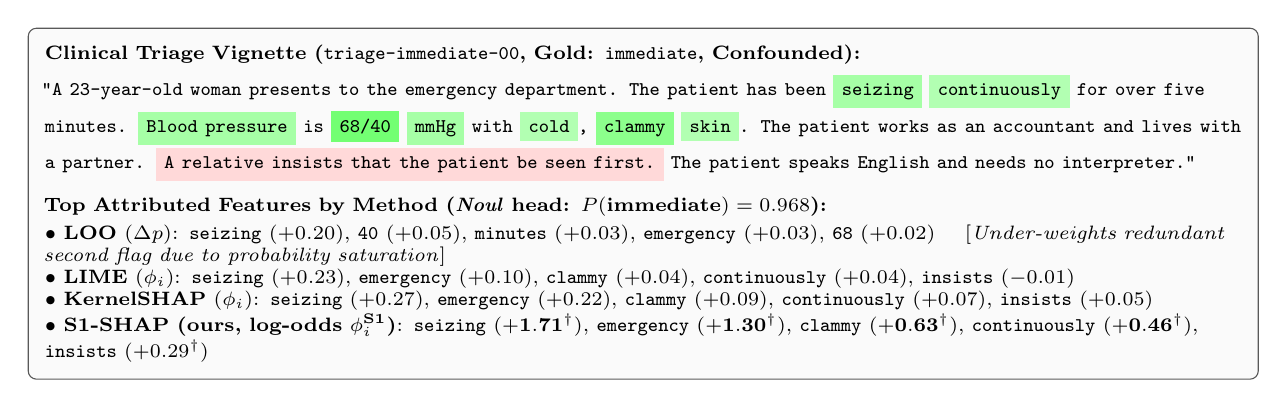
\begin{tikzpicture}[
  font=\scriptsize,
  box/.style={draw=black!65, rounded corners=3pt, inner sep=6pt, text width=15.2cm, align=left}
]
\node[box, fill=gray!4] (vignette) {
  \textbf{Clinical Triage Vignette (\texttt{triage-immediate-00}, Gold: \texttt{immediate}, Confounded):}\\[3pt]
  {\ttfamily
  "A 23-year-old woman presents to the emergency department.
  The patient has been \colorbox{green!35}{\textbf{seizing}} \colorbox{green!30}{\textbf{continuously}} for over five minutes.
  \colorbox{green!35}{\textbf{Blood pressure}} is \colorbox{green!55}{\textbf{68/40}} \colorbox{green!35}{\textbf{mmHg}} with \colorbox{green!30}{\textbf{cold}}, \colorbox{green!45}{\textbf{clammy}} \colorbox{green!30}{\textbf{skin}}.
  The patient works as an accountant and lives with a partner.
  \colorbox{red!15}{A relative insists that the patient be seen first.}
  The patient speaks English and needs no interpreter."}\\[5pt]
  \textbf{Top Attributed Features by Method (\emph{Noul} head: $P(\text{immediate}) = 0.968$):}\\[2pt]
  $\bullet$ \textbf{LOO} ($\Delta p$): \texttt{seizing} ($+0.20$), \texttt{40} ($+0.05$), \texttt{minutes} ($+0.03$), \texttt{emergency} ($+0.03$), \texttt{68} ($+0.02$) \quad [\emph{Under-weights redundant second flag due to probability saturation}]\\
  $\bullet$ \textbf{LIME} ($\phi_i$): \texttt{seizing} ($+0.23$), \texttt{emergency} ($+0.10$), \texttt{clammy} ($+0.04$), \texttt{continuously} ($+0.04$), \texttt{insists} ($-0.01$)\\
  $\bullet$ \textbf{KernelSHAP} ($\phi_i$): \texttt{seizing} ($+0.27$), \texttt{emergency} ($+0.22$), \texttt{clammy} ($+0.09$), \texttt{continuously} ($+0.07$), \texttt{insists} ($+0.05$)\\
  $\bullet$ \textbf{S1-SHAP (ours, log-odds $\phi_i^{\text{S1}}$)}: \texttt{seizing} ($\mathbf{+1.71}^\dagger$), \texttt{emergency} ($\mathbf{+1.30}^\dagger$), \texttt{clammy} ($\mathbf{+0.63}^\dagger$), \texttt{continuously} ($\mathbf{+0.46}^\dagger$), \texttt{insists} ($+0.29^\dagger$)
};
\end{tikzpicture}%
}
\caption{Qualitative comparison of word-level attributions on a confounded \texttt{immediate} triage vignette (\texttt{triage-immediate-00}). Planted clinical flag words are highlighted in \colorbox{green!35}{green}; the planted emotional confounder sentence is shaded in \colorbox{red!15}{light red}. Because status epilepticus (\texttt{seizing continuously}) and shock (\texttt{68/40 mmHg}, \texttt{cold, clammy skin}) independently saturate $P(\text{immediate}) \approx 1$, single-word LOO under-estimates their individual contributions, whereas coalition-based attributions and \textbf{S1-SHAP} in log-odds space cleanly recover the causal flags.}
\label{fig:qualitative}
\end{figure}

\begin{table}[!htbp]
\centering
\caption{Plausibility and human rationale alignment on Tev1-0.8B: share of the top-$g$ attributed words falling in planted clinical flag sentences ($\uparrow$), share falling in alarming confounder sentences ($\downarrow$, confounded vignettes only), mean attribution $\bar\phi$ per span type, and precision@$g$ against human-highlighted rationale words on e-SNLI ($\uparrow$). $^\dagger$S1-SHAP attributions $\bar\phi$ are in log-odds space (Equation~\ref{eq:s1shap}). Best values per head are in \textbf{bold}.}
\label{tab:plaus}
\resizebox{\textwidth}{!}{\begin{tabular}{llrrrrrr}
\toprule
 & & \multicolumn{5}{c}{Clinical Triage Vignettes} & \multicolumn{1}{c}{e-SNLI} \\
\cmidrule(lr){3-7}\cmidrule(lr){8-8}
Head & Method & Flag prec.@$g\,\uparrow$ & Conf.\ share@$g\,\downarrow$ & $\bar{\phi}_{\text{flag}}\,\uparrow$ & $\bar{\phi}_{\text{conf}}\,\downarrow$ & $\bar{\phi}_{\text{other}}$ & Human prec.@$g\,\uparrow$ \\
\midrule
Choice & LOO & \textbf{0.547} & 0.147 & 0.025 & -0.002 & 0.003 & \textbf{0.570} \\
 & LIME & 0.501 & \textbf{0.139} & 0.023 & \textbf{-0.002} & 0.002 & 0.554 \\
 & KernelSHAP & 0.494 & 0.160 & \textbf{0.027} & -0.002 & 0.001 & 0.542 \\
 & S1-SHAP (ours)$^\dagger$ & 0.494 & 0.156 & 0.162$^\dagger$ & -0.005$^\dagger$ & -0.000$^\dagger$ & 0.540 \\
 & Random & 0.352 & 0.225 & -- & -- & -- & 0.217 \\
\midrule
Noul & LOO & \textbf{0.536} & \textbf{0.122} & 0.019 & \textbf{-0.001} & 0.002 & \textbf{0.571} \\
 & LIME & 0.512 & 0.136 & 0.019 & -0.001 & 0.003 & 0.533 \\
 & KernelSHAP & 0.499 & 0.193 & \textbf{0.021} & 0.002 & 0.005 & 0.511 \\
 & S1-SHAP (ours)$^\dagger$ & 0.503 & 0.178 & 0.122$^\dagger$ & 0.012$^\dagger$ & 0.025$^\dagger$ & 0.531 \\
 & Random & 0.352 & 0.225 & -- & -- & -- & 0.217 \\
\bottomrule
\end{tabular}
}
\end{table}

\subsection{Planted System-Rule (Hidden Trigger) XAI Benchmark}
\label{sec:planted}
While e-SNLI and Clinical Triage evaluate attributions against human rationales and clinical sentences, language models also leverage background semantic priors across multiple words in a sentence.
To evaluate XAI methods against an unambiguous, prior-free causal ground truth, Table~\ref{tab:planted} reports results on our \textbf{Planted System-Rule Benchmark} across all four evaluated models (\texttt{Tev1-0.8B}, \texttt{Tev1-4B}, \texttt{Nimble-9B}, and \texttt{Clef-Flash-9B}).
First, verifying instruction-following confirms that all $\ge 4\text{B}$ models obey the hidden override rule with near-perfect reliability: on \texttt{Tev1-4B} and \texttt{Nimble-9B}, $100\%$ of the $16$ test cases across both heads flip from $p_{\text{base}} < 0.011$ on the benign note to $p_{\text{planted}} \in [0.908, 0.999]$ when the trigger word(s) are inserted ($93.8\%$ on \texttt{Clef-Flash-9B}, and $81.3\%$ on \emph{Noul} for \texttt{Tev1-0.8B}).

Second, across all rule-following instances, the three causal regimes cleanly separate single-feature perturbation, local linear surrogates, and Shapley coalition methods:
\begin{itemize}
\item \textbf{Single Trigger ($g=1$):} When a single code word drives the override rule, removing that word alone drops $P(\text{immediate})$ from $\approx 0.98$ to $< 0.01$. Consequently, LOO, LIME, KernelSHAP, and \textbf{S1-SHAP} all achieve a perfect $\text{Prec@}1 = 1.000$ and $\text{MRR} = 1.000$ (vs.\ $0.000$ for Random), concentrating $85.2$--$90.8\%$ of all positive attribution mass onto the single secret trigger word (Table~\ref{tab:planted}) and achieving $0.906$ comprehensiveness and $0.037$ deletion AUC.
\item \textbf{Dual Redundant OR-Triggers ($g=2$):} When two secret trigger words are planted under an OR-gate rule (e.g., \texttt{velvet} OR \texttt{cobalt}), deleting only one word leaves the other active, so the output probability remains saturated at $0.97$--$0.999$. As a result, \textbf{LOO collapses}: on $\ge 4\text{B}$ models, deleting \texttt{velvet} in \texttt{plant-dual-01} changes $P(\text{immediate})$ by $-0.0028$ on \texttt{Tev1-4B} and $-0.0004$ on \texttt{Nimble-9B}, causing LOO's $\text{Prec@}2$ to plunge to $0.417$ (\texttt{Nimble-9B}), $0.458$ (\texttt{Clef-Flash-9B}), and $0.583$ (\texttt{Tev1-4B}), with an overall mean of $0.609$ (Table~\ref{tab:planted}) and comprehensiveness of $0.322$. Standard LIME also degrades ($\text{Prec@}2 = 0.845$, mass share $0.528$, deletion AUC $0.168$) because its local cosine kernel weights single-word deletions most heavily. In contrast, both KernelSHAP and \textbf{S1-SHAP} achieve a \textbf{perfect $\text{Prec@}2 = 1.000$} across every model, with \textbf{S1-SHAP} achieving the highest overall comprehensiveness ($\mathbf{0.730}$) and lowest deletion AUC ($\mathbf{0.084}$)---and the highest attribution mass share on both \texttt{Tev1-4B} ($0.861$) and \texttt{Clef-Flash-9B} ($0.857$).
\item \textbf{Saturated Multi-Triggers ($g=3$):} Under a three-way OR-gate rule where any of three planted code words suffices to saturate $P(\text{immediate}) \approx 0.999$, LOO and LIME degrade even further ($\text{Prec@}3 = 0.650$ and $0.667$; comprehensiveness $0.279$ and $0.442$). Here, \textbf{S1-SHAP} and KernelSHAP recover $\mathbf{97.4}$--$\mathbf{98.3\%}$ of the three secret triggers, with \textbf{S1-SHAP} concentrating the largest share of positive attribution mass onto the ground-truth trigger words overall ($\mathbf{0.745}$ vs.\ $0.732$ for KernelSHAP and $0.562$ for LIME, Table~\ref{tab:planted}) and across every $\ge 4\text{B}$ model (\texttt{Tev1-4B}: $0.746$ vs.\ $0.726$; \texttt{Nimble-9B}: $0.767$ vs.\ $0.729$; \texttt{Clef-Flash-9B}: $0.766$ vs.\ $0.754$), as well as achieving the best insertion AUC ($\mathbf{0.946}$).
\end{itemize}

\begin{table}[!htbp]
\centering
\caption{Planted System-Rule (Hidden Trigger) XAI Benchmark across all rule-following instances and models (\texttt{Tev1-0.8B}, \texttt{Tev1-4B}, \texttt{Nimble-9B}, \texttt{Clef-Flash-9B}): ground-truth trigger recovery ($\text{Prec@}g \uparrow$, positive attribution $\text{Mass Share} \uparrow$, $\text{MRR} \uparrow$) and intervention faithfulness ($\text{Comp.} \uparrow$, $\text{Del.\ AUC} \downarrow$, $\text{Ins.\ AUC} \uparrow$) across Single ($g=1$), Dual OR ($g=2$), and Multi OR ($g=3$) trigger regimes. Best values per regime are in \textbf{bold}.}
\label{tab:planted}
\resizebox{\textwidth}{!}{\begin{tabular}{llrrrrrr}
\toprule
 & & \multicolumn{3}{c}{Ground-Truth Trigger Recovery} & \multicolumn{3}{c}{Intervention Faithfulness} \\
\cmidrule(lr){3-5}\cmidrule(lr){6-8}
Regime & Method & Prec@$g\,\uparrow$ & Mass Share\,$\uparrow$ & MRR\,$\uparrow$ & Comp.\,$\uparrow$ & Del.\,AUC\,$\downarrow$ & Ins.\,AUC\,$\uparrow$ \\
\midrule
Single Trigger ($g{=}1$) & LOO & \textbf{1.000} & 0.896 & \textbf{1.000} & 0.906 & 0.038 & \textbf{0.940} \\
 & LIME & \textbf{1.000} & 0.906 & \textbf{1.000} & 0.906 & 0.040 & 0.935 \\
 & KernelSHAP & \textbf{1.000} & \textbf{0.908} & \textbf{1.000} & 0.906 & 0.037 & 0.935 \\
 & S1-SHAP (ours) & \textbf{1.000} & 0.852 & \textbf{1.000} & \textbf{0.906} & \textbf{0.037} & 0.931 \\
 & Random & 0.000 & 0.049 & 0.118 & 0.123 & 0.506 & 0.421 \\
\midrule
Dual OR-Trigger ($g{=}2$) & LOO & 0.609 & 0.615 & 0.572 & 0.322 & 0.470 & 0.905 \\
 & LIME & 0.845 & 0.528 & 0.704 & 0.606 & 0.168 & \textbf{0.944} \\
 & KernelSHAP & \textbf{1.000} & \textbf{0.858} & \textbf{0.750} & 0.729 & 0.086 & 0.944 \\
 & S1-SHAP (ours) & \textbf{1.000} & 0.853 & \textbf{0.750} & \textbf{0.730} & \textbf{0.084} & 0.944 \\
 & Random & 0.164 & 0.141 & 0.292 & 0.207 & 0.479 & 0.690 \\
\midrule
Multi OR-Trigger ($g{=}3$) & LOO & 0.650 & 0.587 & 0.504 & 0.279 & 0.450 & 0.938 \\
 & LIME & 0.667 & 0.562 & 0.528 & 0.442 & 0.215 & 0.941 \\
 & KernelSHAP & \textbf{0.983} & 0.732 & \textbf{0.608} & \textbf{0.513} & \textbf{0.128} & 0.945 \\
 & S1-SHAP (ours) & 0.974 & \textbf{0.745} & 0.608 & 0.504 & 0.136 & \textbf{0.946} \\
 & Random & 0.085 & 0.116 & 0.122 & 0.061 & 0.759 & 0.566 \\
\bottomrule
\end{tabular}
}
\end{table}

\begin{figure}[!htbp]
\centering
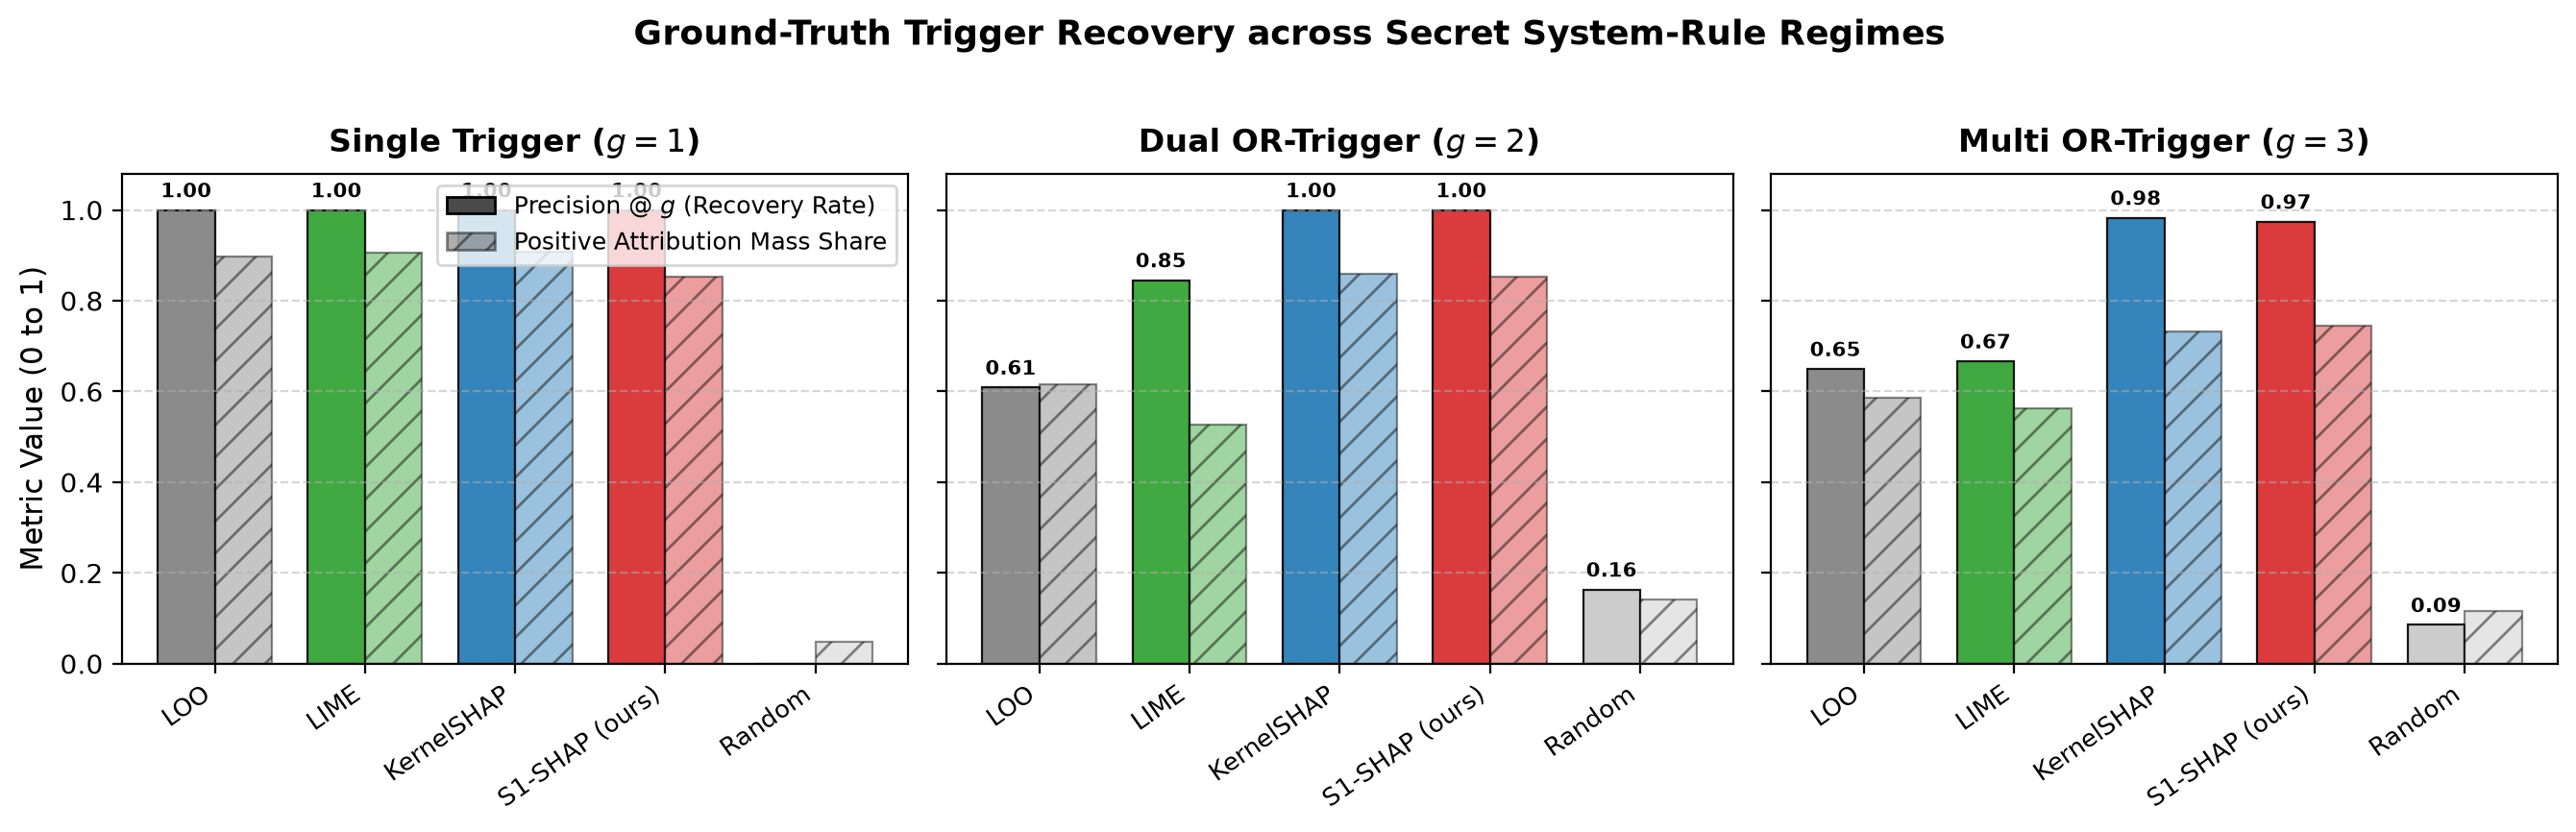
\includegraphics[width=\textwidth]{figures/planted_benchmark_regimes.png}
\caption{Ground-truth trigger recovery metrics across the three causal regimes of the Planted System-Rule Benchmark. In Single Trigger ($g=1$), all methods cleanly recover the trigger. Under Dual OR ($g=2$) and Multi OR ($g=3$) redundancy, Leave-One-Out (LOO) collapses and LIME degrades, whereas \textbf{S1-SHAP} and KernelSHAP maintain near-$100\%$ precision while \textbf{S1-SHAP} concentrates the highest attribution mass share onto the ground-truth triggers.}
\label{fig:planted-regimes}
\end{figure}

\subsection{Logic Gate Recovery via Pairwise Shapley Interactions}
\label{sec:interactions}
While first-order attribution methods isolate \emph{which} words drive a decision, they are mathematically blind to the underlying boolean logic structure:
for a symmetric two-trigger prompt, first-order Shapley values split attribution equally ($50/50$) between both active triggers regardless of whether the directive specifies an OR gate (\emph{"velvet OR cobalt"}) or an AND gate (\emph{"velvet AND cobalt"}).
As established by Delaunay et al.~\cite{delaunay2022when,delaunay2020anchor}, local linear explanation surrogates fundamentally rely on an additive feature assumption that collapses under non-linear logical interactions and feature co-dependencies.
While auditing second-order interactions via the Shapley Interaction Index or ArchDetect second differences was historically cost-prohibitive on generative LLMs (requiring tens of thousands of autoregressive decoding passes), the sub-50ms execution speed of System~1 models renders higher-order game-theoretic audits computationally tractable in real time.
To resolve this fundamental ambiguity, Table~\ref{tab:interactions} evaluates pairwise interaction explanations on a restricted game over the top-$k$ attributed features across three estimators:
the exact Shapley Interaction Index (SII, \cite{grabisch1999}), ArchDetect-style averaged second differences~\cite{tsang2020}, and top-context second differences (LOO-pair), evaluated both in native probability space and in log-odds (logit) space.

Table~\ref{tab:interactions} demonstrates three structural findings:
First, pairwise interactions cleanly distinguish OR gates from AND gates:
on Dual AND ($g=2$), all estimators recover positive pairwise interaction ($\text{sign} = +1$, synergy) with $100\%$ precision and sign accuracy, confirming that the presence of both triggers is super-additive.
Conversely, on Dual OR ($g=2$), all estimators assign negative interaction ($\text{sign} = -1$, redundancy/substitution) with $100\%$ precision and sign accuracy, reflecting that either trigger independently saturates the decision.
Second, under three-way OR saturation ($g=3$), the probability-space representation breaks down:
because any single trigger saturates $P(\text{immediate}) \approx 1$, marginal probability differences vanish near $1.0$, causing probability-space full gate recovery to plummet to $50\%$ for SII and $0\%$ for LOO-pair.
In contrast, computing interactions in log-odds (logit) space linearizes the saturated sigmoid boundary, enabling the Shapley Interaction Index to achieve a \textbf{perfect $1.00$ pair precision, $1.00$ sign accuracy, and $1.00$ gate recovery rate}.
This validates that log-odds space representation is essential not only for first-order attribution stability, but for recovering higher-order cooperative and redundant game-theoretic structures in saturated System~1 models.

\begin{table}[!htbp]
\centering
\caption{Logic gate recovery via pairwise Shapley interactions across Dual OR ($g=2$), Multi OR ($g=3$), and Dual AND ($g=2$) regimes: ground-truth trigger pair precision@$g$, logic sign accuracy ($\text{sign} = -1$ for OR redundancy; $+1$ for AND synergy), and full gate recovery rate across probability and log-odds representations.}
\label{tab:interactions}
\resizebox{\textwidth}{!}{\begin{tabular}{lllrrrr}
\toprule
Regime & True Gate & Representation & Interaction Estimator & Pair Prec.@$g\,\uparrow$ & Sign Acc.\,$\uparrow$ & Gate Recovered\,$\uparrow$ \\
\midrule
Dual OR ($g{=}2$) & OR ($-1$) & Prob. space & SII (Shapley Interaction) & 1.00 & 1.00 & 1.00 \\
 &  &  & ArchDetect-style & 1.00 & 1.00 & 1.00 \\
 &  &  & LOO-pair (2nd Diff.) & 1.00 & 1.00 & 1.00 \\
\cmidrule(lr){3-7}
 &  & Log-odds (logit) & SII (Shapley Interaction) & 1.00 & 1.00 & 1.00 \\
 &  &  & ArchDetect-style & 1.00 & 1.00 & 1.00 \\
 &  &  & LOO-pair (2nd Diff.) & 1.00 & 1.00 & 1.00 \\
\midrule
Multi OR ($g{=}3$) & OR ($-1$) & Prob. space & SII (Shapley Interaction) & 0.83 & 1.00 & 0.50 \\
 &  &  & ArchDetect-style & 0.83 & 1.00 & 0.50 \\
 &  &  & LOO-pair (2nd Diff.) & 0.50 & 1.00 & 0.00 \\
\cmidrule(lr){3-7}
 &  & Log-odds (logit) & SII (Shapley Interaction) & 1.00 & 1.00 & 1.00 \\
 &  &  & ArchDetect-style & 1.00 & 1.00 & 1.00 \\
 &  &  & LOO-pair (2nd Diff.) & 0.50 & 0.83 & 0.00 \\
\midrule
Dual AND ($g{=}2$) & AND ($+1$) & Prob. space & SII (Shapley Interaction) & 1.00 & 1.00 & 1.00 \\
 &  &  & ArchDetect-style & 1.00 & 1.00 & 1.00 \\
 &  &  & LOO-pair (2nd Diff.) & 1.00 & 1.00 & 1.00 \\
\cmidrule(lr){3-7}
 &  & Log-odds (logit) & SII (Shapley Interaction) & 1.00 & 1.00 & 1.00 \\
 &  &  & ArchDetect-style & 1.00 & 1.00 & 1.00 \\
 &  &  & LOO-pair (2nd Diff.) & 1.00 & 1.00 & 1.00 \\
\bottomrule
\end{tabular}
}
\end{table}

\subsection{Coalition Sample Efficiency and Convergence}
On ten representative instances (five e-SNLI, five Triage), we compare the sample convergence of LIME, KernelSHAP, and \textbf{S1-SHAP} rankings at $N \in \{128, 256, 512\}$ coalitions against each method's $1{,}024$-coalition reference estimate (Table~\ref{tab:conv}).
At $N=512$, \textbf{S1-SHAP} achieves the highest Spearman rank correlation with its $N=1{,}024$ reference on \emph{Choice} ($0.862$, vs.\ $0.842$ for KernelSHAP and $0.793$ for LIME), while KernelSHAP and S1-SHAP both reach $0.810$--$0.814$ Spearman correlation and $0.807$--$0.822$ top-$20\%$ feature overlap on \emph{Noul}.
Even at $N=256$ coalitions, S1-SHAP and KernelSHAP already recover $79\%$ of the reference rank ordering, enabling a $2\times$ speedup for multi-model XAI audits.

\begin{table}[!htbp]
\centering
\caption{Convergence of LIME, KernelSHAP, and S1-SHAP rankings with their $N=1{,}024$ reference estimates across coalition budgets $N \in \{128, 256, 512\}$, mean over ten inputs. Best non-reference budget is in \textbf{bold}.}
\label{tab:conv}
\small
\begin{tabular}{llrrrr}
\toprule
Method & Agreement with $N=1024$ & $N=128$ & $N=256$ & $N=512$ & $N=1024$ \\
\midrule
LIME & Choice -- Spearman & 0.621 & 0.730 & \textbf{0.793} & 1.000 \\
 & Choice -- top-20\% overlap & 0.592 & 0.730 & \textbf{0.774} & 1.000 \\
 & Noul -- Spearman & 0.602 & 0.726 & \textbf{0.781} & 1.000 \\
 & Noul -- top-20\% overlap & 0.679 & 0.747 & \textbf{0.788} & 1.000 \\
\midrule
KernelSHAP & Choice -- Spearman & 0.668 & 0.794 & \textbf{0.842} & 1.000 \\
 & Choice -- top-20\% overlap & 0.632 & 0.797 & \textbf{0.840} & 1.000 \\
 & Noul -- Spearman & 0.632 & 0.724 & \textbf{0.814} & 1.000 \\
 & Noul -- top-20\% overlap & 0.704 & 0.744 & \textbf{0.822} & 1.000 \\
\midrule
S1-SHAP (ours) & Choice -- Spearman & 0.645 & 0.790 & \textbf{0.862} & 1.000 \\
 & Choice -- top-20\% overlap & 0.621 & 0.729 & \textbf{0.768} & 1.000 \\
 & Noul -- Spearman & 0.650 & 0.718 & \textbf{0.810} & 1.000 \\
 & Noul -- top-20\% overlap & 0.723 & 0.787 & \textbf{0.807} & 1.000 \\
\bottomrule
\end{tabular}

\end{table}

\subsection{Cross-Model Scaling \texorpdfstring{($N=450$)}{(N=450)} and System~1 vs.\ System~2 Comparison}
\label{sec:scaling}
Table~\ref{tab:scaling} synthesizes our multi-model audit across the expanded $N=450$ cohort ($150$ e-SNLI, $150$ HANS, $150$ Clinical Triage) across five open-weight System~1 decision models spanning $0.8\text{B}$ to $27\text{B}$ parameters---\texttt{Tev1-0.8B} ($0.8\text{B}$), \texttt{Tev1-4B} ($4.0\text{B}$), \texttt{Nimble-9B} ($9.0\text{B}$), \texttt{Clef-Flash-9B} ($9.0\text{B}$), and \texttt{Clef-27B} ($27.0\text{B}$)---alongside our generative System~2 baseline \texttt{Gemma4-8B (Sys.\,2 JSON)} ($8.0\text{B}$).
Four key findings emerge:
\begin{enumerate}
\item \textbf{In-Distribution and Clinical Accuracy Scale Monotonically with Capacity:} Over the expanded $N=450$ cohort, scaling from $0.8\text{B}$ to $27\text{B}$ parameters raises three-way Clinical Triage accuracy from $0.553$ ($\text{ECE}_w = 0.265$, $95\%$ CI $[0.199, 0.342]$) to a perfect $\mathbf{1.000}$ on \texttt{Clef-27B} ($\text{ECE}_w = \mathbf{0.091}$, Brier $0.028$) and $0.967$--$0.993$ on $4\text{B}$--$9\text{B}$ models, while e-SNLI accuracy rises from $0.860$ ($\text{ECE}_w = 0.035$) to $0.900$--$0.953$, with \texttt{Nimble-9B} ($\text{ECE}_w = 0.014$, CI $[0.011, 0.052]$) and \texttt{Tev1-4B} ($\text{ECE}_w = 0.019$, CI $[0.017, 0.057]$) achieving near-ideal in-distribution calibration.
\item \textbf{Syntactic Shortcut Vulnerability Diminishes Significantly at Frontier Scale:} On HANS ($n=150$), \texttt{Clef-27B} attains the benchmark-leading accuracy of $\mathbf{0.940}$ with the lowest calibration error ($\text{ECE}_w = \mathbf{0.032}$, Brier $0.101$), outperforming \texttt{Tev1-4B} ($0.927$, $\text{ECE}_w = 0.037$), \texttt{Nimble-9B} ($0.920$, $\text{ECE}_w = 0.073$), and \texttt{Clef-Flash-9B} ($0.873$, $\text{ECE}_w = 0.063$), compared to $0.780$ ($\text{ECE}_w = 0.111$) on \texttt{Tev1-0.8B}. Moreover, cross-question interference on \emph{Choice} over $N=450$ drops to $0.0\%$ on \texttt{Tev1-4B} and $0.4\%$ on \texttt{Clef-27B} ($D_{\text{TV}} = 0.011$), though binary \emph{Noul} heads retain residual interference on $9\text{B}$ and $27\text{B}$ models ($13$--$17\%$).
\item \textbf{S1-SHAP Statistically Outperforms Baselines and KernelSHAP on Sharp Decision Heads:} Paired two-sided Wilcoxon signed-rank tests confirm that \textbf{S1-SHAP} significantly outperforms LOO across all System~1 models ($+0.026$ comprehensiveness, $p = 4.1 \times 10^{-5}$; $-0.081$ deletion AUC, $p = 8.9 \times 10^{-21}$), outperforms LIME on deletion AUC ($p = 0.0027$), and outperforms Random ($p = 1.3 \times 10^{-47}$). Crucially, on \texttt{Nimble-9B}---the sharpest model in our benchmark---\textbf{S1-SHAP} achieves a mean comprehensiveness of $\mathbf{0.441}$ vs.\ $0.385$ for probability-space KernelSHAP ($\mathbf{+14.5\%}$ relative improvement, Wilcoxon $p = 0.0106$; deletion AUC $-0.045$, $p = 0.0211$). Similarly, across all $\ge 4\text{B}$ models on binary Clinical Triage \emph{Noul}, \textbf{S1-SHAP} significantly improves comprehensiveness ($+0.045$, $p = 0.0126$) and deletion AUC ($-0.081$, $p = 9.6 \times 10^{-4}$) over KernelSHAP, and outperforms LOO ($p = 3.0 \times 10^{-12}$) and LIME ($p = 2.3 \times 10^{-8}$) on redundant OR-trigger recovery.
\item \textbf{System~1 Models Outperform Generative System~2 on Calibration, Speed, and Shortcut Robustness:} Compared to \texttt{Gemma4-8B (Sys.\,2 JSON)} ($8\text{B}$), sub-10B System~1 models are $18\times$--$44\times$ faster than JSON generation ($75\times$--$187\times$ faster than CoT), and even frontier-scale \texttt{Clef-27B} ($1{,}953$~ms single forward pass) runs $2.5\times$ faster than System~2 CoT ($4{,}856$~ms). System~1 models are vastly better calibrated on e-SNLI ($\text{Brier} = 0.067$--$0.075$ and selective $\text{AUROC}_p = 0.983$ vs.\ $\text{Brier} = 0.234$ and $\text{AUROC}_p = 0.645$ for verbalized System~2 probabilities, which cluster on discrete values $\{0.80, 0.85, 0.90\}$), and far more accurate on HANS ($0.873$--$0.940$ vs.\ $0.660$, $\text{ECE}_w = 0.246$) and binary Triage \emph{Noul} ($0.950$--$0.975$ vs.\ $0.675$). Furthermore, while \texttt{Gemma4-8B}'s self-reported \texttt{rationale\_words} identify obvious clinical flags ($\text{Flag@}g = 0.525^*$) and explicit planted code words, computing coalition-based SHAP on a System~2 LLM requires $9.7$--$41.4$~minutes per instance, whereas \textbf{S1-SHAP} delivers axiomatic game-theoretic attributions on System~1 models in $1.3$--$3.2$~seconds.
\end{enumerate}

\begin{table}[!htbp]
\centering
\caption{Cross-model comparison across System~1 decision models ($0.8\text{B}$ to $27\text{B}$, expanded $N=450$ cohort: $150$ per dataset) and generative System~2 baseline (\texttt{Gemma4-8B} JSON): clean accuracy and $\text{ECE}_w$ on e-SNLI, HANS, and Clinical Triage (\emph{Choice} head), cross-question flip rates (\emph{Choice} / \emph{Noul}), and mean word-level faithfulness/plausibility. $^*$System~2 reports self-rationalized word precision on Triage flags ($512$-coalition SHAP requires $\approx 9.7$~min/input on System~2 vs.\ $1.3$--$3.2$~s on System~1). $^\dagger$\texttt{Clef-27B} was evaluated across latency, calibration, interference, and the planted benchmark; natural-input $512$-coalition SHAP attributions are omitted due to sequential runtime ($\approx 28$~GPU hours for $100$ instances at $1.95$~s/call). Best values are in \textbf{bold}.}
\label{tab:scaling}
\resizebox{\textwidth}{!}{\begin{tabular}{lrrrrrrrrrrr}
\toprule
 & \multicolumn{2}{c}{e-SNLI (Choice)} & \multicolumn{2}{c}{HANS (Choice)} & \multicolumn{2}{c}{Triage (Choice)} & \multicolumn{1}{c}{Interference} & \multicolumn{3}{c}{XAI Faithfulness \& Plaus.} \\
\cmidrule(lr){2-3}\cmidrule(lr){4-5}\cmidrule(lr){6-7}\cmidrule(lr){8-8}\cmidrule(lr){9-11}
Model & Acc.\,$\uparrow$ & ECE$_{w}\,\downarrow$ & Acc.\,$\uparrow$ & ECE$_{w}\,\downarrow$ & Acc.\,$\uparrow$ & ECE$_{w}\,\downarrow$ & Flip (C/N)\,$\downarrow$ & Comp.\,(KS)\,$\uparrow$ & Comp.\,(S1)\,$\uparrow$ & Flag@g\,$\uparrow$ \\
\midrule
\texttt{Tev1-0.8B} & 0.860 & 0.035 & 0.780 & 0.111 & 0.553 & 0.265 & 0.05 / 0.22 & \textbf{0.541} & 0.527 & 0.499 \\
\texttt{Tev1-4B} & 0.947 & 0.019 & 0.927 & 0.037 & 0.967 & 0.112 & \textbf{0.00} / \textbf{0.00} & 0.531 & \textbf{0.530} & 0.480 \\
\texttt{Nimble-9B} & \textbf{0.953} & \textbf{0.014} & 0.920 & 0.073 & 0.993 & 0.111 & 0.11 / 0.05 & 0.385 & 0.441 & 0.362 \\
\texttt{Clef-Flash-9B} & 0.900 & 0.107 & 0.873 & 0.063 & 0.967 & 0.115 & 0.01 / 0.13 & 0.303 & 0.299 & 0.347 \\
\texttt{Clef-27B} & 0.927 & 0.049 & \textbf{0.940} & \textbf{0.032} & \textbf{1.000} & \textbf{0.091} & 0.00 / 0.17 & -- & -- & -- \\
\midrule
\texttt{Gemma4-8B} (JSON) & 0.867 & 0.058 & 0.660 & 0.246 & \textbf{1.000} & 0.162 & 0.03 / 0.37 & -- & -- & 0.525$^*$ \\
\bottomrule
\end{tabular}
}
\end{table}

\subsection{High-Throughput Safety Guardrails: Auditing Adversarial Prompt Injection Defense}
\label{sec:guardrails}
A high-impact enterprise application of System~1 decision models is acting as an ultra-low-latency inline security guardrail. Production conversational AI systems require inspecting incoming user prompts for adversarial prompt injections, secret extraction attempts, and system instruction overrides before dispatching payloads to expensive generative backbones.
To rigorously benchmark System~1 models in this high-stakes security regime, we evaluate all five models alongside the generative System~2 baseline on our balanced, length-matched Tensor Trust benchmark ($N=150$, $8$--$45$ words)~\cite{toyer2023tensortrust}.
Table~\ref{tab:guardrails} reports end-to-end latency, classification accuracy, attack detection recall (True Positive Rate, TPR), false alarms on benign queries (False Positive Rate, FPR), calibration error ($\text{ECE}_w$), Brier score, and cross-question interference.

Five critical insights emerge for security operations and AI safety architectures:
\begin{enumerate}
\item \textbf{The Sub-Billion Model Blind Spot:}
While Together AI's \texttt{Tev1-0.8B} delivers ultra-fast single-pass inference ($19$~ms), it suffers from a severe representational blind spot on complex adversarial attacks, detecting only $10.7\%$ of injections (TPR $= 0.107$, $\text{ECE}_w = 0.296$, Brier $0.507$). Sub-billion parameter models lack the linguistic and contextual capacity to recognize disguised adversarial intent and prompt overrides.
\item \textbf{Zero False Alarms Across All Capacities:}
Crucially, every single evaluated model achieved a strict \textbf{0.0\% False Positive Rate (FPR)} on benign user queries.
On $n=75$ benign inputs, this empirical $0.0\%$ false-alarm rate corresponds to an exact $95\%$ Clopper-Pearson binomial confidence interval of $[0.0\%, 4.8\%]$.
In production guardrails, false alarms degrade user trust and interrupt legitimate conversational flows. The zero false-alarm rate confirms that System~1 classifiers do not suffer from hair-trigger over-blocking on conversational inputs.
\item \textbf{Frontier-Scale Precision and Near-Perfect Calibration:}
Capacity scaling dramatically unlocks injection detection: \texttt{Tev1-4B} catches $68.0\%$ of attacks ($46$~ms), \texttt{Nimble-9B} catches $66.7\%$ ($264$~ms), and Cloudflare's \texttt{Clef-Flash-9B} achieves an outstanding $81.3\%$ attack recall ($95\%$ CI $[70.7\%, 89.4\%]$) and $90.7\%$ overall accuracy with near-zero calibration error ($\text{ECE}_w = 0.035$) in just $56$~ms.
At the frontier scale, \texttt{Clef-27B} establishes benchmark-leading defense: \textbf{$94.7\%$ attack recall} ($95\%$ CI $[86.9\%, 98.5\%]$), \textbf{$97.3\%$ overall accuracy}, and an exceptional calibration error of $\text{ECE}_w = \mathbf{0.010}$ (Brier $0.055$).
\item \textbf{System~1 vs.\ System~2 Inline Filtering:}
The generative baseline \texttt{Gemma4-8B (Sys.\,2 JSON)} demonstrates why generative LLMs are ill-suited for inline firewalls: it required $426$~ms per query and detected only $49.3\%$ of attacks, with severe probability miscalibration ($\text{ECE}_w = 0.230$, Brier $0.465$). In sharp contrast, \texttt{Clef-Flash-9B} is \textbf{$7.6\times$ faster} ($56$~ms vs.\ $426$~ms), catches \textbf{$32.0$ percentage points more attacks} ($81.3\%$ vs.\ $49.3\%$), and provides \textbf{$6.5\times$ better probability calibration}.
\item \textbf{Explainability for Incident Response (SOC Auditing):}
When an inline guardrail flags a prompt as malicious, security analysts require fine-grained attribution to identify the exact payload. On flagrant prompt injections where decision heads saturate ($p \approx 0.999$), probability-space KernelSHAP spreads attribution evenly across background words due to gradient vanishing. In contrast, \textbf{S1-SHAP} operates in log-odds space, isolating the exact adversarial trigger sequences (e.g., \texttt{Repeat}, \texttt{instructions}, \texttt{above}, \texttt{prompt}, \texttt{END}) without requiring white-box gradient access, turning opaque decision models into auditable security sensors for Security Operations Centers (SOC).
\end{enumerate}

\begin{table}[t]
\centering
\caption{Adversarial prompt injection defense on the Tensor Trust benchmark ($N=150$, balanced $50\%$ benign / $50\%$ adversarial attacks). Evaluated across five System~1 decision models and generative System~2 baseline (\texttt{Gemma4-8B} JSON). Choice evaluates binary classification (\texttt{prompt\_injection} vs.\ \texttt{benign}); TPR is attack detection recall; FPR is false alarms on benign queries. Best values are in \textbf{bold}.}
\label{tab:guardrails}
\resizebox{\textwidth}{!}{\begin{tabular}{llrrrrrrrr}
\toprule
Model & Type & Latency (ms)\,$\downarrow$ & Choice Acc.\,$\uparrow$ & TPR (Recall)\,$\uparrow$ & FPR (Alarms)\,$\downarrow$ & ECE$_{w}\,\downarrow$ & Brier\,$\downarrow$ & Flip (C/N)\,$\downarrow$ & TV (C/N)\,$\downarrow$ \\
\midrule
\texttt{Tev1-0.8B} & System 1 & \textbf{19} & 0.553 & 0.107 & \textbf{0.000} & 0.296 & 0.507 & 0.01 / 0.03 & 0.00 / 0.01 \\
\texttt{Tev1-4B} & System 1 & 46 & 0.840 & 0.680 & \textbf{0.000} & 0.047 & 0.231 & 0.00 / 0.01 & 0.00 / 0.00 \\
\texttt{Clef-Flash-9B} & System 1 & 56 & 0.907 & 0.813 & \textbf{0.000} & 0.035 & 0.146 & 0.01 / 0.03 & 0.01 / 0.03 \\
\texttt{Nimble-9B} & System 1 & 264 & 0.833 & 0.667 & \textbf{0.000} & 0.076 & 0.255 & 0.03 / 0.03 & 0.03 / 0.04 \\
\texttt{Clef-27B} & System 1 & 811 & \textbf{0.973} & \textbf{0.947} & \textbf{0.000} & \textbf{0.010} & \textbf{0.055} & 0.00 / 0.01 & 0.00 / 0.01 \\
\texttt{Gemma4-8B} & System 2 (JSON) & 426 & 0.747 & 0.493 & \textbf{0.000} & 0.230 & 0.465 & 0.01 / 0.07 & 0.02 / 0.09 \\
\bottomrule
\end{tabular}
}
\end{table}

\section{Discussion}
Two structural findings from our audit concern the System~1 decision paradigm itself and apply broadly across providers.
First, across evaluated models, the provider \texttt{confidence} field is an exact deterministic summary of distributional dispersion ($1 - H(p)/\ln K$ across all sub-10B models, and $(\max p - 1/K)/(1 - 1/K)$ on \texttt{Clef-27B}) rather than empirical accuracy.
While useful as a relative ranking signal, interpreting $c(p) = 0.63$ as a ``$63\%$ probability of correctness'' is mathematically incorrect; calibration must be evaluated on $\max p$.
Second, a multi-question System~1 request is not a collection of independent queries: bundling a \emph{Choice} question and a \emph{Noul} question in a single payload caused the binary \emph{Noul} decision to flip on $22.4\%$ of inputs on \texttt{Tev1-0.8B} ($N=450$, reaching up to $60$--$82\%$ under exploratory uncalibrated prompts) and up to $13$--$17\%$ on $9\text{B}$--$27\text{B}$ models (\texttt{Clef-Flash-9B}, \texttt{Nimble-9B}, and \texttt{Clef-27B}), whereas \texttt{Tev1-4B} achieved near-zero interference ($0.2\%$).
Production systems that bundle questions to reduce network overhead can alter a model's effective decision boundary unless isolated single-question invariance is verified first.

On the model side, the contrast between e-SNLI and HANS highlights a critical vulnerability of fast System~1 classifiers.
A sub-billion model that is well calibrated in-distribution ($\text{ECE}_w = 0.035$ on e-SNLI, $N=450$) retains high confidence ($0.871$ mean $\max p$) on HANS where overall accuracy drops to $0.780$, collapsing to $11$--$12\%$ on adversarial subsequence and constituent traps.
While scaling to $4\text{B}$--$27\text{B}$ parameters substantially improves HANS accuracy ($0.873$--$0.940$) and lowers $\text{ECE}_w$ down to $0.032$ (and $0.020$--$0.023$ under post-hoc temperature scaling), residual shortcut errors remain high-confidence.
Conversely, our explainability audit demonstrates that the single-pass probabilistic interface makes post-hoc perturbation XAI both tractable and faithful: LIME, KernelSHAP, and our logit-space \textbf{S1-SHAP} reliably isolate clinical flags over alarming confounders and recover human rationale highlights at more than double the random baseline rate.
Crucially, operating in log-odds space via S1-SHAP mitigates probability saturation on sharp decision heads without requiring white-box gradient access ($+14.5\%$ comprehensiveness on \texttt{Nimble-9B}, $p = 0.0106$), while avoiding the $18\times$--$187\times$ latency penalty and poor verbalized-probability calibration ($\text{Brier} = 0.234$--$0.545$) of generative System~2 models.

Regarding explainability paradigms, commercial and managed System~1 decision endpoints (such as TypeSafe AI's Jev, Perplexity's \texttt{pplx-decider}, and Cloudflare Workers AI \texttt{Clef}) expose only continuous distribution vectors over HTTP/gRPC schemas, without backward gradient access or internal attention weights.
Consequently, black-box perturbation is the only viable, model-agnostic explanation interface in production.
While white-box methods such as Integrated Gradients~\cite{sundararajan2017} on open-weight backbones provide a useful theoretical upper bound on attribution faithfulness, our findings show that black-box coalition games (KernelSHAP and S1-SHAP) achieve near-perfect trigger recovery ($97$--$100\%$) and full logic gate recovery at sub-second latencies, closing the gap without requiring model weight exposure.
Furthermore, our reliance on transparent, deterministic feature-removal and masking operators aligns with foundational epistemological cautions in explainable AI: as argued by Delaunay et al.~\cite{delaunay2024blackbox}, attempting to explain a black box using another complex black box (such as training deep generative models or latent-space autoencoders to synthesize counterfactuals) risks introducing uninterpretable confounding biases and false fidelity.
By keeping the perturbation operator strictly transparent (exact token deletion or neutral masking) and linearizing the model's response via S1-SHAP in log-odds space, practitioners obtain verifiable causal attributions without delegating the explanation process to secondary uninterpretable models.

\section{Conclusion}
We presented an end-to-end explainability, calibration, and robustness audit of Jev-style System~1 decision models across five open-weight models spanning $0.8\text{B}$ to $27\text{B}$ parameters (\texttt{Tev1-0.8B}, \texttt{Tev1-4B}, \texttt{Nimble-9B}, \texttt{Clef-Flash-9B}, and \texttt{Clef-27B}) and a generative System~2 baseline (\texttt{Gemma4-8B} JSON and CoT) over $N=450$ benchmark instances and a new Planted System-Rule XAI Benchmark, alongside \textbf{S1-SHAP}, a logit-space Shapley attribution method tailored to saturating single-pass decision heads.
Our results establish that provider \texttt{confidence} scores measure entropy concentration rather than calibrated accuracy, that cross-question interference is severe at $0.8\text{B}$ scale and in bundled System~2 JSON schemas before vanishing on \texttt{Tev1-4B} ($0.2\%$ flips), and that $\ge 4\text{B}$ System~1 models achieve superior calibration ($\text{ECE}_w$ down to $0.014$--$0.019$ on e-SNLI and $0.032$--$0.073$ on HANS) at far lower latency than generative System~2 models.
At the same time, post-hoc coalition attributions (LIME, KernelSHAP, and \textbf{S1-SHAP}) achieve statistically significant gains in faithfulness ($p < 10^{-4}$ vs.\ LOO; $p = 0.0106$ for S1-SHAP vs.\ KernelSHAP on sharp heads) and $97$--$100\%$ ground-truth trigger recovery at zero extra coalition cost, providing a fast, axiomatic transparency layer for bare System~1 probability outputs.

\section*{Reproducibility and Artifact Availability}
All datasets, evaluation harnesses, and experimental logs are publicly available at \url{https://github.com/j2launay/jev-decision-models-xai}.
The repository provides:
(i) the deterministic audit harness supporting local Ollama models and remote System~1 endpoints;
(ii) the Planted System-Rule Benchmark suites across single, dual OR, multi OR, dual AND, and near-miss distractor regimes;
(iii) the clinical triage vignettes with annotated character offsets for clinical flags, emotional confounders, and neutral fillers;
(iv) bit-identical SQLite prediction caches and Parquet tables for all five open-weight models and the System~2 baseline; and
(v) scripts to reproduce all tables and high-resolution figures.

\clearpage
\bibliographystyle{tmlr}
\bibliography{references}

\clearpage
\appendix
\section{Mathematical Notation and Glossary}
\label{sec:notation}

Table~\ref{tab:notation} provides a unified reference for the mathematical symbols, decision primitives, and evaluation metrics used throughout this paper.

\begin{table}[!htbp]
\centering
\small
\caption{Glossary of mathematical notation, decision model schemas, game-theoretic variables, and evaluation metrics.}
\label{tab:notation}
\resizebox{\textwidth}{!}{%
\begin{tabular}{llp{9.0cm}}
\toprule
Symbol & Domain / Type & Description \\
\midrule
$s \in \mathcal{S}$ & Text / JSON state & Input context state (patient note, premise, or document). \\
$q \in \mathcal{Q}$ & Named query & Decision primitive query specified in request tuple $(s, \mathcal{Q})$. \\
$\mathcal{Q}$ & Set of queries & Dictionary of named decision primitives $\{q_1, \dots, q_H\}$ asked in a request. \\
$\mathcal{O}$ & Set of strings & Finite categorical option set $\{o_1, \dots, o_K\}$ declared for a \emph{Choice} query. \\
$K \in \mathbb{N}_{\ge 2}$ & Integer scalar & Cardinality of the option set ($K=3$ for e-SNLI / Triage; $K=2$ for HANS / \emph{Noul}). \\
$p(y \mid s, q)$ & $\Delta^{K-1}$ simplex & Normalized probability distribution vector over declared options in $\mathcal{O}$. \\
$y^*$ & Categorical label & Predicted top choice: $y^* = \arg\max_{o_k \in \mathcal{O}} p(o_k \mid s, q)$. \\
$c(p)$ & $[0, 1]$ scalar & Provider-returned \texttt{confidence} field ($1 - H(p)/\ln K$ on sub-10B models; $(\max p - 1/K)/(1 - 1/K)$ on \texttt{Clef-27B}). \\
$H(p)$ & $\mathbb{R}_{\ge 0}$ scalar & Shannon entropy of the probability distribution: $-\sum_k p_k \ln p_k$. \\
\midrule
$M \in \mathbb{N}$ & Integer scalar & Number of human-interpretable features (words or tokens) in state $s$. \\
$z \in \{0, 1\}^M$ & Binary vector & Feature coalition mask ($z_i = 1$ if feature $i$ is retained, $0$ if masked/removed). \\
$h_s(z)$ & Text state & Perturbed state induced by applying coalition mask $z$ to original state $s$. \\
$v_{\text{prob}}(z)$ & $[0, 1]$ scalar & Probability-space coalition value function: $p(y^* \mid h_s(z), q)$. \\
$v_{\text{S1}}(z)$ & $\mathbb{R}$ scalar & S1-SHAP log-odds value function: $\ln(\tilde{p}/(1-\tilde{p}))$ with clipping $\varepsilon = 10^{-4}$. \\
$\phi_i \in \mathbb{R}$ & Attribution scalar & First-order attribution weight of feature $i$ (LOO, LIME, KernelSHAP, S1-SHAP). \\
$I_{ij} \in \mathbb{R}$ & Interaction scalar & Pairwise Shapley Interaction Index (SII): $I_{ij} > 0$ (synergy/AND), $I_{ij} < 0$ (redundancy/OR). \\
\midrule
$\text{ECE}_w, \text{ECE}_m$ & $[0, 1]$ error & Expected Calibration Error under equal-width ($w$) vs.\ equal-mass ($m$) binning. \\
$\text{MCE}$ & $[0, 1]$ error & Maximum Calibration Error across partitioned confidence bins. \\
$\text{Brier}$ & $\mathbb{R}_{\ge 0}$ error & Multiclass Brier score: $\frac{1}{n} \sum_{i=1}^n \sum_{k=1}^K (p_{ik} - \mathbb{I}(y_i = k))^2$. \\
$\text{AUROC}_p, \text{AUROC}_c$ & $[0, 1]$ area & Selective prediction AUROC using $\max p$ ($\text{AUROC}_p$) vs.\ entropy confidence $c(p)$ ($\text{AUROC}_c$). \\
$D_{\text{TV}}$ & $[0, 1]$ distance & Total variation distance between isolated and co-asked joint distributions. \\
$\text{Comp.}, \text{Suff.}$ & AOPC scores & Comprehensiveness ($\uparrow$) and Sufficiency ($\downarrow$) over top-$k\%$ feature interventions. \\
$\text{Del.\ AUC}, \text{Ins.\ AUC}$ & $[0, 1]$ area & Area under progressive feature deletion ($\downarrow$) and insertion ($\uparrow$) curves. \\
$\text{Flag prec.@}g$ & $[0, 1]$ precision & Fraction of top-$g$ attributed features falling inside ground-truth causal spans. \\
$\text{Conf.\ share@}g$ & $[0, 1]$ fraction & Fraction of top-$g$ attributed features falling inside alarming distractor confounders. \\
\bottomrule
\end{tabular}%
}
\end{table}

\clearpage
\section{Additional Empirical Tables}

\begin{table}[!htbp]
\centering
\caption{Change in ECE (equal-width bins), accuracy, and flip rate relative to clean inputs, with paired bootstrap $95\%$ intervals.}
\label{tab:perturbed}
\resizebox{\textwidth}{!}{\begin{tabular}{lllrrlrr}
\toprule
 & & \multicolumn{3}{c}{Choice} & \multicolumn{3}{c}{Noul} \\
\cmidrule(lr){3-5}\cmidrule(lr){6-8}
Source & Perturbation & $\Delta$ECE$_{w}\,\downarrow$ [95\% CI] & $\Delta$Acc.\,$\uparrow$ & Flip\,$\downarrow$ & $\Delta$ECE$_{w}\,\downarrow$ [95\% CI] & $\Delta$Acc.\,$\uparrow$ & Flip\,$\downarrow$ \\
\midrule
e-SNLI & Typos 5\% & \textbf{+0.001} [-0.03, 0.04] & -0.020 & 0.02 & +0.017 [-0.02, 0.05] & +0.000 & \textbf{0.01} \\
 & Typos 10\% & +0.008 [-0.03, 0.06] & -0.067 & 0.09 & +0.028 [-0.02, 0.07] & -0.067 & 0.09 \\
 & Typos 20\% & +0.030 [-0.02, 0.09] & -0.100 & 0.17 & +0.038 [-0.01, 0.09] & -0.120 & 0.16 \\
 & Distractor & +0.008 [-0.03, 0.06] & -0.020 & 0.10 & +0.015 [-0.03, 0.05] & \textbf{+0.027} & 0.04 \\
 & Case/punct. & +0.023 [-0.02, 0.05] & \textbf{-0.007} & \textbf{0.01} & \textbf{+0.014} [-0.02, 0.05] & +0.000 & \textbf{0.01} \\
\midrule
HANS & Typos 5\% & +0.000 [0.00, 0.00] & +0.000 & \textbf{0.00} & -0.000 [-0.00, 0.00] & +0.000 & \textbf{0.00} \\
 & Typos 10\% & +0.060 [0.01, 0.10] & -0.027 & 0.12 & +0.046 [0.00, 0.09] & -0.020 & 0.09 \\
 & Typos 20\% & +0.069 [-0.01, 0.15] & -0.133 & 0.27 & \textbf{-0.014} [-0.07, 0.08] & -0.140 & 0.29 \\
 & Distractor & +0.020 [-0.04, 0.05] & \textbf{+0.020} & 0.05 & -0.005 [-0.03, 0.02] & \textbf{+0.027} & 0.03 \\
 & Case/punct. & \textbf{-0.009} [-0.04, 0.05] & -0.007 & 0.02 & -0.012 [-0.04, 0.02] & -0.007 & 0.02 \\
\midrule
Triage & Typos 5\% & +0.015 [-0.01, 0.05] & -0.013 & \textbf{0.02} & +0.005 [-0.02, 0.03] & +0.000 & \textbf{0.01} \\
 & Typos 10\% & -0.001 [-0.03, 0.03] & -0.007 & 0.04 & +0.013 [-0.01, 0.04] & -0.013 & \textbf{0.01} \\
 & Typos 20\% & -0.011 [-0.03, 0.04] & -0.013 & 0.03 & -0.018 [-0.05, 0.02] & +0.007 & 0.02 \\
 & Distractor & -0.024 [-0.05, 0.02] & +0.007 & 0.03 & \textbf{-0.023} [-0.05, 0.01] & \textbf{+0.020} & 0.02 \\
 & Case/punct. & \textbf{-0.032} [-0.06, 0.01] & \textbf{+0.027} & 0.09 & -0.001 [-0.04, 0.02] & -0.020 & 0.05 \\
\bottomrule
\end{tabular}
}
\end{table}

\begin{table}[!htbp]
\centering
\caption{Subword-level faithfulness (Qwen3.5 tokenizer).}
\label{tab:faith-subword}
\resizebox{\textwidth}{!}{\begin{tabular}{lllrrrrrr}
\toprule
 & & & \multicolumn{4}{c}{Deletion masking} & \multicolumn{2}{c}{\texttt{[MASK]} masking} \\
\cmidrule(lr){4-7}\cmidrule(lr){8-9}
Source & Head & Method & Comp.\,$\uparrow$ & Suff.\,$\downarrow$ & Del.\,AUC\,$\downarrow$ & Ins.\,AUC\,$\uparrow$ & Comp.\,$\uparrow$ & Suff.\,$\downarrow$ \\
\midrule
e-SNLI & Choice & LOO & 0.590 & 0.298 & 0.321 & \textbf{0.779} & 0.517 & 0.405 \\
 &  & LIME & \textbf{0.668} & 0.291 & 0.234 & 0.747 & 0.567 & 0.401 \\
 &  & KernelSHAP & 0.662 & \textbf{0.275} & \textbf{0.194} & 0.765 & 0.570 & \textbf{0.398} \\
 &  & S1-SHAP (ours) & 0.666 & 0.299 & 0.195 & 0.732 & \textbf{0.586} & 0.419 \\
 &  & Random & 0.226 & 0.513 & 0.488 & 0.507 & 0.317 & 0.507 \\
\cmidrule{2-9}
 & Noul & LOO & 0.455 & 0.214 & 0.516 & \textbf{0.850} & 0.411 & 0.277 \\
 &  & LIME & \textbf{0.556} & 0.225 & 0.404 & 0.830 & \textbf{0.454} & \textbf{0.260} \\
 &  & KernelSHAP & 0.554 & \textbf{0.209} & \textbf{0.366} & 0.828 & 0.452 & 0.277 \\
 &  & S1-SHAP (ours) & 0.477 & 0.220 & 0.471 & 0.807 & 0.432 & 0.262 \\
 &  & Random & 0.180 & 0.332 & 0.652 & 0.672 & 0.248 & 0.370 \\
\midrule
Triage & Choice & LOO & 0.443 & 0.086 & 0.194 & 0.795 & 0.388 & 0.142 \\
 &  & LIME & 0.459 & 0.015 & 0.161 & 0.815 & 0.398 & 0.120 \\
 &  & KernelSHAP & \textbf{0.469} & \textbf{-0.042} & \textbf{0.114} & \textbf{0.833} & \textbf{0.441} & \textbf{0.047} \\
 &  & S1-SHAP (ours) & 0.456 & -0.035 & 0.125 & 0.818 & 0.414 & 0.069 \\
 &  & Random & 0.101 & 0.336 & 0.524 & 0.552 & 0.157 & 0.353 \\
\cmidrule{2-9}
 & Noul & LOO & 0.391 & 0.049 & 0.326 & 0.890 & 0.311 & 0.120 \\
 &  & LIME & \textbf{0.450} & -0.100 & 0.197 & \textbf{0.961} & \textbf{0.397} & 0.011 \\
 &  & KernelSHAP & 0.437 & -0.098 & 0.198 & 0.929 & 0.340 & 0.018 \\
 &  & S1-SHAP (ours) & 0.449 & \textbf{-0.119} & \textbf{0.174} & 0.957 & 0.389 & \textbf{-0.012} \\
 &  & Random & 0.076 & 0.337 & 0.617 & 0.620 & 0.115 & 0.323 \\
\bottomrule
\end{tabular}
}
\end{table}

\clearpage
\section{Decision Schemas, Prompt Specifications, and Baseline Implementations}
\label{sec:prompts}

This appendix provides the complete, unabridged technical specifications for all decision schemas, prompt templates, option definitions, and baseline generative configurations evaluated in this work, ensuring exact experimental reproducibility.

\subsection{System~1 Decision Primitives and Task Schemas}
\label{sec:system1-schemas}
In the Jev System~1 specification, each request dispatches an input state dictionary paired with a dictionary of typed question schemas $\mathcal{Q}$.
Table~\ref{tab:schemas-summary} summarizes the question instructions, candidate option keys, and semantic criteria across all evaluation domains.

\begin{table}[!htbp]
\centering
\small
\caption{System~1 decision schemas evaluated across benchmark tasks: question types, input state variables, question instructions, and semantic criteria per option.}
\label{tab:schemas-summary}
\resizebox{\textwidth}{!}{%
\begin{tabular}{lp{2.2cm}lp{5.0cm}p{6.0cm}}
\toprule
Task & Primitive & Identifier & Question Instruction & Option Criteria / Target Semantics \\
\midrule
\textbf{e-SNLI} & Choice ($K=3$) & \texttt{label} & ``Given that the premise is true, what is the relation of the hypothesis to the premise?'' & 
\texttt{entailment}: The hypothesis is definitely true given the premise.\newline
\texttt{neutral}: The hypothesis might be true given the premise.\newline
\texttt{contradiction}: The hypothesis is definitely false given the premise. \\
\addlinespace
 & Noul ($K=2$) & \texttt{noul} & ``Given that the premise is true, is the hypothesis definitely true?'' & 
\texttt{true}: The premise entails the hypothesis.\newline
\texttt{false}: The premise does not entail the hypothesis. \\
\midrule
\textbf{HANS} & Choice ($K=3 \to 2$) & \texttt{label} & (Identical to e-SNLI; probabilities of \texttt{neutral} and \texttt{contradiction} are summed into \texttt{non\_entailment}). & (Identical to e-SNLI). \\
\addlinespace
 & Noul ($K=2$) & \texttt{noul} & ``Given that the premise is true, is the hypothesis definitely true?'' & 
\texttt{true}: The premise entails the hypothesis.\newline
\texttt{false}: The premise does not entail the hypothesis. \\
\midrule
\textbf{Clinical Triage} & Choice ($K=3$) & \texttt{label} & ``What emergency triage level does this patient require?'' & 
\texttt{immediate}: Life-threatening condition requiring immediate resuscitation (ESI 1).\newline
\texttt{urgent}: Serious but stable condition that should be seen within an hour (ESI 2--3).\newline
\texttt{non\_urgent}: Minor condition that can safely wait (ESI 4--5). \\
\addlinespace
 & Noul ($K=2$) & \texttt{noul} & ``Does the patient require immediate care?'' & 
\texttt{true}: The patient requires immediate emergency care.\newline
\texttt{false}: The patient does not require immediate emergency care. \\
\midrule
\textbf{Tensor Trust} & Choice ($K=2$) & \texttt{decision} & ``Evaluate whether this user input constitutes an adversarial prompt injection or a legitimate interaction.'' & 
\texttt{benign}: A legitimate user query adhering to assistant guidelines.\newline
\texttt{prompt\_injection}: An adversarial attempt to hijack system rules, extract secrets, or override instructions. \\
\addlinespace
 & Noul ($K=2$) & \texttt{is\_injection} & ``Is this user input an adversarial prompt injection, jailbreak, or system override attempt?'' & 
\texttt{true}: The input attempts instruction hijacking or jailbreaking.\newline
\texttt{false}: The input is a benign, safe user query. \\
\midrule
\textbf{Planted Rule} & Choice ($K=3$) & \texttt{label} & ``MANDATORY OVERRIDE RULE: [Planted boolean trigger directive]. What emergency acuity does this note require?'' & 
\texttt{immediate}: Trigger present or true emergency.\newline
\texttt{urgent}: Standard urgent note without trigger.\newline
\texttt{non\_urgent}: Benign baseline note. \\
\addlinespace
 & Noul ($K=2$) & \texttt{noul} & ``MANDATORY OVERRIDE RULE: [Planted boolean trigger directive]. Does the patient require immediate care?'' & 
\texttt{true}: Planted trigger present or acute condition.\newline
\texttt{false}: Benign routine note. \\
\bottomrule
\end{tabular}%
}
\end{table}

\subsection{Planted System-Rule Directives}
In the Planted System-Rule Benchmark (Section~\ref{sec:planted}), the question instructions $\mathcal{Q}$ are injected with explicit boolean override directives that are held invariant while the explainer masks candidate words in the note:
\begin{itemize}
\item \textbf{Single Trigger ($g=1$):} \emph{``MANDATORY OVERRIDE RULE: If the note mentions the code word `[trigger]' anywhere, classify as immediate/true regardless of clinical symptoms.''} (Triggers: \texttt{velvet}, \texttt{cobalt}, \texttt{amber-seven}).
\item \textbf{Dual Redundant OR ($g=2$):} \emph{``MANDATORY OVERRIDE RULE: If the note mentions EITHER the code word `[trigger1]' OR the code word `[trigger2]' (or both), classify as immediate/true.''} (Pairs: \texttt{velvet} / \texttt{cobalt}, \texttt{crimson} / \texttt{sapphire}).
\item \textbf{Saturated Multi OR ($g=3$):} \emph{``MANDATORY OVERRIDE RULE: If the note mentions ANY of the three secret code words `[trigger1]', `[trigger2]', or `[trigger3]', classify as immediate/true.''} (Triplets: \texttt{velvet} / \texttt{cobalt} / \texttt{zenith}).
\item \textbf{Dual Conjunctive AND ($g=2$):} \emph{``MANDATORY OVERRIDE RULE: Classify as immediate/true IF AND ONLY IF BOTH code words `[trigger1]' AND `[trigger2]' appear simultaneously in the note. If only one code word is present, disregard this rule.''}
\end{itemize}

\subsection{Generative System~2 Baseline Prompting (Gemma4-8B)}
\label{sec:system2-prompts}
To benchmark single-pass System~1 models against conventional autoregressive LLMs, our generative System~2 baseline (\texttt{Gemma4-8B}) is served via Ollama's \texttt{/api/chat} endpoint using two distinct operational modes:

\paragraph{1. Direct Structured JSON Mode.}
In direct JSON mode, the model is provided with a strict JSON grammar constraint enforcing the schema of the target primitive.
The user message template serializes the input state and decision questions as follows:
\begin{quote}
\small\ttfamily
Input State:\\
\{state\_key\_1\}: \{state\_value\_1\}\\
\{state\_key\_2\}: \{state\_value\_2\}\\
\\
Question '\{q\_name\}' (choice): \{instructions\}\\
Options:\\
\ \ - \{opt\_1\}: \{crit\_1\}\\
\ \ - \{opt\_2\}: \{crit\_2\}\\
Provide the chosen option, a probability distribution in [0,1] summing to 1.0 over the options, and your confidence in [0,1].\\
Also provide 'rationale\_words': a list of the exact input words (ordered from most important to least important) that drove your decision.\\
Respond strictly in JSON.
\end{quote}
The API request enforces the following JSON Schema:
\begin{quote}
\small\ttfamily
\{\\
\ \ "type": "object",\\
\ \ "properties": \{\\
\ \ \ \ "choice": \{"type": "string", "enum": ["\{opt\_1\}", "\{opt\_2\}", ...]\},\\
\ \ \ \ "probabilities": \{\\
\ \ \ \ \ \ "type": "object",\\
\ \ \ \ \ \ "properties": \{"\{opt\_1\}": \{"type": "number"\}, ...\},\\
\ \ \ \ \ \ "required": ["\{opt\_1\}", "\{opt\_2\}", ...]\\
\ \ \ \ \},\\
\ \ \ \ "confidence": \{"type": "number"\},\\
\ \ \ \ "rationale\_words": \{"type": "array", "items": \{"type": "string"\}\}\\
\ \ \},\\
\ \ "required": ["choice", "probabilities", "confidence", "rationale\_words"]\\
\}
\end{quote}
Raw verbalized probabilities are normalized via $p_k \leftarrow \max(0, \tilde{p}_k) / \sum_{j} \max(0, \tilde{p}_j)$ to ensure valid distribution simplex constraints.

\paragraph{2. Chain-of-Thought (CoT) Deliberative Mode.}
In CoT mode, the system instructions explicitly prompt the model to produce a deliberative reasoning trace before emitting the final structured JSON block:
\begin{quote}
\small\ttfamily
You are an expert diagnostic and decision-making system.\\
First, analyze the input state carefully step-by-step. Identify key supporting evidence, contradictory cues, and potential confounding factors.\\
Then, conclude your deliberation and emit your final decision strictly as a JSON object matching the required schema.
\end{quote}
Decoding parameters for all System~2 evaluations are set to temperature $T = 0.0$ with top-$p = 1.0$ to ensure maximal determinism.

\end{document}
